%======================================================================
\chapter{Identification problems in plasticity}\label{ch:id}
%======================================================================
% Sources: A. Constantinescu, "Identification and inverse problems in solid
% mechanics", AMAS Lecture Notes (Warsaw, 2003), Part I, Ch. 4-5; talks
% "Inverse problems in solid mechanics" (Beijing 2005, Tokyo 2011);
% Tardieu and Constantinescu, Inverse Problems 16 (2000); Constantinescu and
% Tardieu, Inverse Problems in Engineering 9 (2001); Lecampion, Constantinescu
% and Nguyen Minh, IJNAMG 26 (2002); Lecampion and Constantinescu, IJNAMG 29
% (2005); Lecampion, Constantinescu and Malinsky, Int. J. Geomech. 6 (2006);
% Michaleris, Tortorelli and Vidal, IJNME 37 (1994).
% Draft of 4 Oct 2026; code in python/examples/ch7 (id_core.py).

\framepart{Outline}
Chapters~\ref{ch:pl}--\ref{ch:pl-cyc} computed the response of a structure
when the constitutive law is known. In practice the law is known only up to a
few parameters, the modulus, the yield stress, the hardening modulus, a
viscosity, and these parameters must be read from experiments: a tension test,
an indentation curve, the convergence of a tunnel, a displacement field
measured by image correlation. This chapter treats the \emph{identification}
of these parameters. The experiment is computed with the methods of the
previous chapters, the computed response is compared with the measured one by
a \emph{cost functional}, and the parameters are those that minimize the cost.

Three questions organize the chapter. What can the data tell, and how can one
see it before minimizing anything? How is the minimization done, with or
without derivatives? And how is the derivative of the cost computed, when the
response comes from a nonlinear, path-dependent computation with contact? The
answer to the last question is the \emph{adjoint state}: one more problem,
linear, solved backward in time, which gives the whole gradient whatever the
number of parameters. Its structure is the familiar one: the adjoint of a
contact problem is a problem on the contact zone that the forward computation
found, and the adjoint of a return map uses the consistent tangent of the
plastic points that the forward computation found. \emph{Only the active
constraints play a role in the differentiation.}

Three model problems carry the chapter: the three-bar truss of
Chapter~\ref{ch:pl-cyc}, now with unknown $(E,\sY,H)$; a membrane indented by
a rigid punch, the simplest model of an indentation test; and a Norton--Hoff
filament in a relaxation test. All the numbers quoted are computed, and the
scripts are printed with the exercises.

\paragraph{By the end of this chapter you should be able to:}
\begin{itemize}
  \item set an identification problem: model, experiment, observations,
  parameters, and say which parameters the experiment can determine;
  \item write a least-squares cost, its Gauss--Newton matrix, and read
  identifiability and uncertainty from the eigenvalues of that matrix;
  \item choose between a derivative-free method (Nelder--Mead), a quasi-Newton
  method (BFGS) and Levenberg--Marquardt, and count their costs;
  \item compute a gradient by finite differences, by direct differentiation and
  by the adjoint state, for a linear problem, a contact problem and an
  elastoplastic evolution;
  \item explain why the adjoint of a contact problem is a linear problem on the
  contact zone, and why the derivative of a return map freezes the plastic
  points;
  \item assemble an identification with today's tools: a finite element code,
  automatic differentiation, and an optimization or calibration driver.
\end{itemize}

\paragraph{Plan of the chapter.} Section~\ref{sec:id-settings} sets the
problem and the three model problems. Section~\ref{sec:id-min} writes it as a
minimization and introduces the sensitivity matrix.
Section~\ref{sec:id-algo} compares the minimization algorithms.
Section~\ref{sec:id-grad} computes gradients for a linear problem,
Section~\ref{sec:id-contact} for a contact problem, and
Section~\ref{sec:id-path} for an elastoplastic or elastoviscoplastic
evolution. Section~\ref{sec:id-tools} shows how the pieces fit together in
present-day software. A summary, exercises with solutions
(page~\pageref{sec:id-exo}) and the references close the chapter. General
references are Bui~\cite{Bui1993id}, Tarantola~\cite{Tarantola2005}, Bonnet and
Constantinescu~\cite{BonnetConstantinescu2005}, Mahnken~\cite{Mahnken2004}
and, for sensitivity analysis, Kleiber et al.~\cite{KleiberEtAl1997}.

\begin{gbox}{Guiding questions}
\begin{enumerate}[itemsep=1pt]
  \item Which parameters can an experiment determine, and with which
  uncertainty? (Sections~\ref{sec:id-settings}--\ref{sec:id-min})
  \item When are derivatives worth computing, and which algorithm uses them
  best? (Section~\ref{sec:id-algo})
  \item How does one differentiate a response computed with contact, plasticity
  and time stepping, at the price of one more computation?
  (Sections~\ref{sec:id-grad}--\ref{sec:id-path})
  \item How do a finite element code, automatic differentiation and an
  optimization library fit together? (Section~\ref{sec:id-tools})
\end{enumerate}
The tools are the Lagrangians and multipliers of Chapter~\ref{ch:var}, the
reciprocity of Chapter~\ref{ch:rg}, the generalized standard materials of
Chapter~\ref{ch:pl}, the return map and its consistent tangent of
Chapter~\ref{ch:pl-num}, the fibre structures of Chapter~\ref{ch:pl-cyc}, and
Newton's method of Appendix~\ref{app:iter}.
\end{gbox}

%======================================================================
\section{Setting an identification problem}\label{sec:id-settings}
\index{identification!setting}\index{inverse problem!identification}%
\subsection{Model, experiment, observations}\label{ssec:id-def}
\index{direct problem}\index{observation map}%
Three kinds of quantities enter an identification, and it pays to keep them
apart.
\begin{itemize}
  \item The \emph{parameters} $\vp=(p_1,\dots,p_{n_p})$ of the constitutive law, in
  an admissible set $\mathcal Q$ (moduli are positive, an exponent is larger than
  one). They are unknown, and they are the same in every experiment made on the
  material.
  \item The \emph{loading} $\ell(t)$, $t\in[0,T]$: everything that the experiment
  imposes, the forces on $S_t$, the displacements on $S_u$, a temperature, the depth
  of a punch, together with the geometry of the specimen. It is the data of the
  direct problem of Chapter~\ref{ch:pl} (box in Section~\ref{ssec:pl-bvp-eq}). It is
  known, and it is chosen by the experimenter: one can repeat the test with
  another loading $\ell^{(2)}$, $\ell^{(3)}$, \dots
  \item The \emph{observations} $\mat{y}$: the quantities that were measured, at the
  instants $t_n$: a force, the displacement of a gauge, a field on a surface. They
  are \emph{other} quantities than the imposed ones. Where a displacement is
  imposed, the reaction force is measured; where a force is imposed, a
  displacement. The loading and the observations together overdetermine the
  boundary data, as the Cauchy data of Chapter~\ref{ch:rg}.
\end{itemize}
Between them stands the \emph{state} $s=(\vu,\sig,\vz)(t)$ of the structure, the
solution of the evolution problem, and an \emph{observation operator}
$\mathcal O$ that extracts the measured quantities from the state: the
displacement of a node, the resultant of the contact pressures, the stress in a
gauge.

\begin{gbox}{Direct and inverse problems}\label{def:id-direct}
\begin{itemize}
  \item \textbf{Direct problem.} Given the parameters $\vp\in\mathcal Q$ and the loading
  $\ell$, compute the state $s(\vp;\ell)$ by solving the evolution problem, and the
  observations
  \begin{equation}\label{eq:id-obsmap}
    \mat{y}(\vp;\ell)=\mathcal O\bigl(s(\vp;\ell)\bigr).
  \end{equation}
  \item \textbf{Inverse problem (identification).} Given the loadings
  $\ell^{(k)}$ of $K$ experiments and the measured observations
  $\mat{y}^{m,(k)}$, find $\vp\in\mathcal Q$ such that
  $\mat{y}(\vp;\ell^{(k)})=\mat{y}^{m,(k)}$, $k=1,\dots,K$.
\end{itemize}
\end{gbox}
\noindent The map $\vp\mapsto\mat{y}(\vp;\ell)$ at a fixed loading is the
\emph{observation map}. To evaluate it once is to run one complete simulation:
for each step $t_n$, the loads $\ell(t_n)$ are applied, the nodal equilibrium is
solved by Newton's method with the return map at the Gauss points (Box~5.3), and
the observations of the step are extracted. The map is nonlinear in $\vp$ even
for a linear material (the displacement of an elastic bar is $FL/(ES)$, not linear
in $E$), and it inherits the path dependence of plasticity: $\mat{y}_n$ depends
on the whole loading up to $t_n$. Several experiments simply stack their
observations; we keep one loading in the notation and write $\mat{y}(\vp)$ when
$\ell$ is fixed.

Hadamard asks three questions of the inverse problem: does a solution exist, is
it unique, does it depend continuously on the data? Measurements are noisy and
models are approximate, so an exact solution rarely exists; the next section
replaces the equation by a minimization. Uniqueness is the question of
\emph{identifiability}, and continuity the question of the uncertainty of the
parameters. Both depend on the loading as much as on the material: the choice of
$\ell$, the design of the experiment, decides what can be identified, and both
can be read on the derivative $\partial\mat{y}/\partial\vp$ before any minimization
is attempted (Section~\ref{ssec:id-sens}).

\paragraph{The filament in a tension test.}
\index{identifiability!tension test}%
The simplest identification is done by hand. A filament with linear
kinematic hardening (Section~\ref{ssec:pl-1d-kin}) is pulled at increasing
strain; the stress is measured (Figure~\ref{fig:id-models}a). The parameters are
$\vp=(E,\sY,H)$, the loading is the strain history $\ell=\varepsilon(t)$, and the
observations are the stresses $\mat{y}=(\sigma(t_n))_n$; computing $\mat{y}(\vp)$ is
running Box~5.1 along the strain history. The curve has two straight branches: the
elastic branch of slope $E$, the yield point at $\sigma=\sY$, and the plastic
branch of slope $E_t=EH/(E+H)$. Three readings give the three parameters:
\[
  E=\text{slope}_1,\qquad \sY=\sigma_{\text{knee}},\qquad
  H=\frac{E\,E_t}{E-E_t}\quad(E_t=\text{slope}_2).
\]
Each part of the curve informs one parameter. A test that stays elastic
determines $E$ and nothing else. And a monotone test cannot tell isotropic
from kinematic hardening: both give the slope $E_t$ in tension; only the
reverse loading separates them, through the Bauschinger effect
(Exercise~\ref{exo:id-q-tension}). The same three lessons, which part of the
data carries which parameter, which parameters never appear, which
parameters appear only together, return in every example of the chapter.

\subsection{Three model problems}\label{ssec:id-models}
\index{model problems (identification)}%
\paragraph{The truss.}
\index{three-bar truss!identification}%
The three-bar truss of Section~\ref{ssec:cy-truss}, with bars of modulus $E$,
yield stress $\sY$ and kinematic hardening modulus $H$, is loaded at its node
by the forces
\[
  Q_1(t)=2.3N_0\sin t,\qquad Q_2(t)=0.8N_0\sin2t,\qquad t\in[0,2\pi],
\]
in 80 steps, with $N_0=S\sY$. The displacement $(u_1,u_2)$ of the node is
measured at every step; the true values are $E=200$\,GPa, $\sY=200$\,MPa,
$H=10$\,GPa, and the measurements are the computed displacements plus a noise
of $1\%$ of their maximum. The bars yield in 38 of the 80 steps, and the plastic
strain reaches $4.2\,\varepsilon_Y$ (Figure~\ref{fig:id-models}b). Here
$\vp=(E,\sY,H)$, the loading is the force history $\ell=(Q_1,Q_2)(t_n)$ at the
node, and the observations are the 160 numbers $\mat{y}=(u_1,u_2)(t_n)$,
$n=1,\dots,80$. Computing $\mat{y}(\vp)$ is the incremental computation of
Chapter~\ref{ch:pl-cyc}: at each step, Newton's method on the two nodal
equilibrium equations, with the return map in each bar, one Gauss point per bar.
The result is a force--displacement loop of a structure
(Figure~\ref{fig:id-truss}a).

\paragraph{Indentation.}
\index{indentation!membrane model}%
An indentation test presses a rigid punch into a body and records the force
$F$ against the depth $U$~\cite{TardieuConstantinescu2000,ConstantinescuTardieu2001b}.
Its simplest model is a membrane of tension $T_m$ resting on an elastic
foundation of modulus $k_f$, on $[-1,1]$ with fixed ends, pressed by a punch of
profile $g(x)=x^2/(2R)$, $R=0.5$ (Figure~\ref{fig:id-indent}a). With the
deflection $u$ positive downwards, the punch imposes $u\ge U-g$, and the
contact zone, where the membrane follows the punch, is unknown
(Figure~\ref{fig:id-models}c). The parameters are $\vp=(k_f,T_m)$, of true values
$(4,1)$; the loading is the sequence of depths $\ell=(U_j)_j$ imposed to the
punch; the observations are the forces on the punch,
$\mat{y}=(F(U_j))_j$. The material is elastic, so the depths are independent:
computing $\mat{y}(\vp)$ is solving one contact problem per depth, for the
deflections of the 79 nodes, and adding the contact forces. Section~\ref{sec:id-contact} uses it to show how
contact enters the gradient.

\paragraph{Relaxation of a Norton--Hoff filament.}
\index{Norton--Hoff law!identification}\index{relaxation test}%
A filament obeys the Norton--Hoff law~\eqref{eq:pl-norton} in one dimension,
\begin{equation}\label{eq:id-norton}
  \sigma=E(\varepsilon-\varepsilon^{vp}),\qquad
  \dot\varepsilon^{vp}=\Bigl\langle\frac{|\sigma|-\sY}{K}\Bigr\rangle^{m}\sign\sigma ,
\end{equation}
with the viscosity $K$ in MPa\,s$^{1/m}$ and the exponent $m$. The strain is
raised to $3\times10^{-3}$ in $10$\,s, held for a time $t_h$, and brought back to
zero in $10$\,s; the stress is measured (Figure~\ref{fig:id-models}d). Here
$\vp=(E,\sY,K,m)$, the loading is the strain history $\ell=\varepsilon(t)$, and
the observations are the stresses $\mat{y}=(\sigma(t_n))_n$. The test is
homogeneous and strain-driven: there is no equilibrium to solve, and computing
$\mat{y}(\vp)$ is the backward Euler update of~\eqref{eq:id-norton} along the
strain history, one scalar nonlinear equation per step
(Figure~\ref{fig:id-norton}a). The true
parameters are $E=200$\,GPa, $\sY=200$\,MPa, $K=500$\,MPa\,s$^{1/5}$, $m=5$. It
is the one-point version of the indentation of an elastoviscoplastic
body~\cite{ConstantinescuTardieu2001b} and of the convergence of a tunnel in
a viscoplastic rock~\cite{LecampionConstantinescuNguyen2002}, where the same
four parameters are identified from field measurements.

\begin{table}[h]
\centering\small
\renewcommand{\arraystretch}{1.2}
\begin{tabular}{@{}>{\raggedright}p{2.1cm}>{\raggedright}p{1.9cm}>{\raggedright}p{2.6cm}>{\raggedright}p{4.6cm}p{2.9cm}@{}}
\toprule
\sffamily problem & \sffamily parameters $\vp$ & \sffamily loading $\ell$ (imposed) & \sffamily computing the state & \sffamily observations $\mat{y}$\\
\midrule
filament, tension & $E$, $\sY$, $H$ & strain $\varepsilon(t)$ & Box~5.1 along the history & stress $\sigma(t_n)$\\
truss & $E$, $\sY$, $H$ & forces $Q_1(t)$, $Q_2(t)$ at the node & nodal equilibrium by Newton (Box~5.3), return map in each bar & displacement $(u_1,u_2)(t_n)$ of the node\\
indentation (membrane) & $k_f$, $T_m$ & depths $U_j$ of the punch & one contact problem~\eqref{eq:id-contact} per depth & force $F(U_j)$ on the punch\\
Norton filament & $E$, $\sY$, $K$, $m$ & strain $\varepsilon(t)$: ramp, hold, unload & backward Euler of~\eqref{eq:id-norton} & stress $\sigma(t_n)$\\
tunnel~\cite{LecampionConstantinescuNguyen2002} & $E$, $\sY$, $K$, $N$ & excavation, lining at $t_l$ & finite elements, Norton--Hoff return map & convergence, pressure cells\\
\bottomrule
\end{tabular}
\caption{Parameters, loading and observations of the identification problems of
the chapter; one evaluation of the observation map $\mat{y}(\vp;\ell)$ is one run
of the computation of the fourth column.}
\label{tab:id-problems}
\end{table}

\begin{figure}[h]
\centering
\begin{tikzpicture}[>=Latex,
  imp/.style={->,very thick,cphi!80!black},
  mes/.style={->,very thick,red!70!black},
  lab/.style={font=\small}]
  % ---------------- (a) filament
  \begin{scope}
    \node[font=\sffamily\bfseries\small,anchor=west] at (-0.4,2.3) {(a) filament, tension};
    \fill[pattern=north east lines] (-0.3,0.55) rectangle (0,1.45);
    \draw[thick] (0,0.55) -- (0,1.45);
    \draw[line width=3pt,gray!60] (0,1) -- (2.6,1);
    \draw[imp] (2.6,1) -- (3.4,1) node[right,lab,cphi!70!black] {$\varepsilon(t)$};
    \node[lab,red!70!black] at (1.3,1.4) {$\sigma(t)$};
    \draw[->] (0,-1.4) -- (3.4,-1.4) node[right,font=\scriptsize] {$\varepsilon$};
    \draw[->] (0,-1.4) -- (0,0.15) node[above,font=\scriptsize] {$\sigma$};
    \draw[thick,red!70!black] (0,-1.4) -- (0.6,-0.4) -- (3.1,-0.05);
    \node[font=\scriptsize] at (0.5,-1.0) {$E$};
    \node[font=\scriptsize,above] at (2.0,-0.2) {$E_t$};
    \draw[dashed,gray] (0,-0.4) node[left,font=\scriptsize,black] {$\sY$} -- (0.6,-0.4);
  \end{scope}
  % ---------------- (b) truss
  \begin{scope}[xshift=8.2cm,yshift=0.4cm,scale=0.6]
    \node[font=\sffamily\bfseries\small,anchor=west] at (-3.6,3.15) {(b) three-bar truss};
    \coordinate (O) at (0,0);
    \coordinate (A) at (-2,-2); \coordinate (B) at (-2,2); \coordinate (C) at (-2,0);
    \foreach \P in {A,B,C}{\fill[pattern=north east lines] ($(\P)+(-0.3,-0.25)$) rectangle ($(\P)+(0,0.25)$);
       \draw[thick] ($(\P)+(0,-0.25)$) -- ($(\P)+(0,0.25)$);}
    \draw[very thick,gray!70] (A) -- (O) node[midway,below right,black,font=\scriptsize] {1};
    \draw[very thick,gray!70] (B) -- (O) node[midway,above right,black,font=\scriptsize] {2};
    \draw[very thick,gray!70] (C) -- (O) node[midway,above,black,font=\scriptsize] {3};
    \foreach \P in {A,B,C,O}{\fill[white,draw=black] (\P) circle (2pt);}
    \draw[imp] (O) -- (1.5,0) node[right,lab,cphi!70!black] {$Q_1(t)$};
    \draw[imp] (O) -- (0,1.5) node[above,lab,cphi!70!black] {$Q_2(t)$};
    \draw[mes] (O) -- (1.0,-1.0) node[below right,lab,red!70!black] {$\vu(t)$};
  \end{scope}
  % ---------------- (c) membrane
  \begin{scope}[yshift=-4.6cm]
    \node[font=\sffamily\bfseries\small,anchor=west] at (-0.4,2.1) {(c) indentation of a membrane};
    \fill[gray!30,domain=-1.1:1.1,samples=40] plot ({\x+3.2},{-0.55+0.45*\x*\x}) -- (4.3,1.0) -- (2.1,1.0) -- cycle;
    \draw[thick,domain=-1.1:1.1,samples=40] plot ({\x+3.2},{-0.55+0.45*\x*\x});
    \foreach \x in {0.4,1.0,...,6.0}{
      \pgfmathsetmacro{\yy}{-0.55*exp(-1.4*(\x-3.2)*(\x-3.2))}
      \draw[spring,gray!70!black] (\x,\yy) -- (\x,-1.6);}
    \fill[pattern=north east lines] (-0.1,-1.75) rectangle (6.5,-1.6);
    \draw (-0.1,-1.6) -- (6.5,-1.6);
    \foreach \x in {0,6.4}{\fill[pattern=north east lines] (\x-0.12,0) rectangle (\x+0.12,0.25);}
    \draw[very thick,cu,domain=-3.2:3.2,samples=80] plot ({\x+3.2},{-0.55*exp(-1.4*\x*\x)});
    \draw[line width=2.2pt,red!70!black] (2.85,-0.53) -- (3.55,-0.53);
    \draw[dashed,gray] (4.4,0) -- (7.1,0);
    \draw[dashed,gray] (3.4,-0.55) -- (7.1,-0.55);
    \draw[<->,thick,cphi!80!black] (6.95,0) -- (6.95,-0.55) node[midway,right,lab,cphi!70!black] {$U$};
    \draw[mes] (3.2,1.0) -- (3.2,1.7) node[right,lab,red!70!black] {$F$};
    \node[lab,cu] at (1.0,0.35) {$T_m$};
    \node[lab] at (-0.45,-0.9) {$k_f$};
  \end{scope}
  % ---------------- (d) Norton relaxation
  \begin{scope}[xshift=8.2cm,yshift=-4.6cm]
    \node[font=\sffamily\bfseries\small,anchor=west] at (-0.6,2.1) {(d) relaxation of a Norton filament};
    \draw[->] (0,0) -- (5.0,0) node[right,font=\scriptsize] {$t$};
    \draw[->] (0,-1.3) -- (0,1.6);
    \draw[very thick,cphi!80!black] (0,0) -- (0.6,1.1) -- (4.0,1.1) -- (4.5,0);
    \node[font=\scriptsize,cphi!70!black,anchor=west] at (0.7,1.3) {imposed $\varepsilon(t)$: ramp, hold $t_h$, unload};
    \draw[very thick,red!70!black,domain=0.6:4.0,samples=40] plot (\x,{0.45+0.4*exp(-1.6*(\x-0.6))});
    \draw[very thick,red!70!black] (0,0) .. controls (0.35,0.75) .. (0.6,0.85);
    \draw[very thick,red!70!black] (4.0,0.45) -- (4.5,-0.95);
    \node[font=\scriptsize,red!70!black,anchor=west] at (1.6,0.25) {measured $\sigma(t)$};
  \end{scope}
\end{tikzpicture}
\caption{The model problems of the chapter: the imposed loading $\ell$ in green,
the observations $\mat{y}$ in red. (a) Filament pulled at an imposed strain, with
the bilinear curve of linear kinematic hardening. (b) The three-bar truss of
Chapter~\ref{ch:pl-cyc} under forces at the node, whose displacement is measured.
(c) A membrane of tension $T_m$ on a foundation of modulus $k_f$, pressed to the
depth $U$ by a rigid punch; the force $F$ is measured; the contact zone (red)
is unknown. (d) Relaxation test on a Norton--Hoff filament: imposed strain history
and measured stress.}
\label{fig:id-models}
\end{figure}

\subsection{What the data can tell}\label{ssec:id-tell}
\index{identifiability}\index{lumped parameters}%
Before any computation, three simple arguments often decide what can be
identified.
\begin{itemize}
  \item \emph{Inactive parts of the model are invisible.} If the plastic
  threshold is never reached, $\sY$ and $H$ do not enter the response at all:
  their derivatives vanish, and no algorithm can find them. In the truss
  loaded by $Q_1=N_0\sin t$ alone, the bars stay elastic, and only $E$ can be
  identified. This is the first appearance of the rule of this chapter:
  only the active constraints count.
  \item \emph{Invariances give lumped parameters.} The membrane model is
  linear in $(k_f,T_m)$: multiplying both by $\lambda$ multiplies the force by
  $\lambda$, at every depth. One depth therefore gives one combination of the
  two parameters, and only the variation of the force with the depth
  separates them. Lecampion et al.~\cite{LecampionConstantinescuMalinsky2006}
  show in the same way that a confinement test on a tight rock determines the
  bulk moduli and one diffusivity $D=kMK/(\mu_fK_u)$, not the permeability $k$
  and the Biot modulus $M$ separately.
  \item \emph{Each part of the history informs some parameters.} In the tension
  test, the elastic branch gives $E$, the knee $\sY$, the plastic branch $H$. In
  indentation, the unloading branch carries the modulus~\cite{ConstantinescuTardieu2001b};
  in a relaxation test, the long times carry the threshold and the short times
  the viscosity. The experiment must be designed so that each parameter is
  active in some part of it.
\end{itemize}
Section~\ref{sec:id-min} turns these arguments into a computation: the
eigenvalues of the Gauss--Newton matrix.

%======================================================================
\section{Identification as a minimization}\label{sec:id-min}
\index{cost functional}\index{least squares!output}%
\subsection{Cost functionals}
The measurements contain noise, and the model is never exact: the equation
$\mat{y}(\vp)=\mat{y}^m$ has no solution in general. It is replaced by the
minimization of a distance between the computed and the measured observations.
\begin{gbox}{Output least squares}\label{def:id-ols}
\begin{equation}\label{eq:id-ols}
  \min_{\vp\in\mathcal Q}\ \mathcal J(\vp),\qquad
  \mathcal J(\vp)=\frac12\sum_{i}\Bigl(\frac{y_i(\vp)-y^m_i}{s_i}\Bigr)^2
  =\frac12\,\norm{\mat{r}(\vp)}^2 ,\qquad
  r_i(\vp)=\frac{y_i(\vp)-y^m_i}{s_i},
\end{equation}
where $s_i$ is the scale of the observation $i$, ideally the standard deviation
of its noise.
\end{gbox}
\noindent The scales make the cost dimensionless and weigh displacements
against forces, or a gauge against another. Lecampion et
al.~\cite{LecampionConstantinescuNguyen2002} weigh the convergences and the
pressures of a tunnel so that both have errors of the same order. With
$s_i$ equal to the standard deviation of independent Gaussian noise,
\eqref{eq:id-ols} is the maximum-likelihood estimate, and its minimum is about
half the number of observations. With the scale $\sY l/E$ of the truss, the noise
is $0.063$ scale units, and $\tfrac12\times160\times0.063^2\approx0.32$ is the
expected minimum for its 160 observations; the computed one is $0.29$.

Two variants are common.
\begin{itemize}
  \item \emph{Regularization} adds $\tfrac\beta2\norm{\vp-\vp_0}^2$, a prior
  guess $\vp_0$ weighted by $\beta$~\cite{Tarantola2005}. It removes the flat
  directions of $\mathcal J$ at the price of a bias towards $\vp_0$.
  \item \emph{Bounds} keep $\vp$ in $\mathcal Q$. At a minimum on the boundary
  the gradient need not vanish; the optimality condition is the variational
  inequality $\nabla\mathcal J(\vp)\cdot(\vq-\vp)\ge0$ for all $\vq\in\mathcal Q$,
  as in~\cite{ConstantinescuTardieu2001b}. Positivity is simplest to enforce by
  minimizing over $\log\vp$, which is done in all the computations of this
  chapter.
\end{itemize}
Energy functionals, which measure the error of the constitutive law instead of
the error of the outputs (the error in constitutive relation of Ladev\`eze and
of Kohn and Vogelius, its modified version of Allix and Feissel, and the
alternating algorithm for elastic moduli), are not treated here.
\draftnote{Energy functionals (CRE, MCRE, alternating algorithm) and full-field
methods (FEMU, VFM) go into a later chapter: first in elasticity, then in
elastoplasticity.}


\subsection{The sensitivity matrix}\label{ssec:id-sens}
\index{sensitivity matrix}\index{Gauss--Newton matrix}%
Expand the residual near a parameter vector $\vp$:
$\mat{r}(\vp+\delta\vp)\approx\mat{r}(\vp)+\mat{S}\,\delta\vp$, with the
\emph{sensitivity matrix}
\begin{equation}\label{eq:id-S}
  \mat{S}=\frac{\partial\mat{r}}{\partial\vp},\qquad
  S_{ij}=\frac1{s_i}\frac{\partial y_i}{\partial p_j}.
\end{equation}
Column $j$ of $\mat{S}$ is the response of the experiment to a small change of
the parameter $p_j$. Then
\begin{equation}\label{eq:id-GN}
  \mathcal J(\vp+\delta\vp)\approx\mathcal J(\vp)+\mat{r}\T\mat{S}\,\delta\vp
  +\tfrac12\,\delta\vp\T\,\mat{S}\T\mat{S}\,\delta\vp ,
\end{equation}
and the gradient is $\nabla\mathcal J=\mat{S}\T\mat{r}$. The matrix
$\mat{S}\T\mat{S}$, the \emph{Gauss--Newton matrix}, is the Hessian of
$\mathcal J$ without the term $\sum_ir_i\nabla^2r_i$, small when the residuals
are small. It is symmetric and positive semi-definite.

\begin{gbox}{The Gauss--Newton matrix decides what can be identified}\label{prop:id-GN}
Let $\lambda_1\le\dots\le\lambda_{n_p}$ be the eigenvalues of $\mat{S}\T\mat{S}$ at the
solution, with the unit eigenvectors $\mat{v}_k$, and let the observations carry
independent noises of standard deviation $s_i$. Then:
\begin{itemize}
  \item a zero eigenvalue is a combination $\mat{v}_k$ of the parameters that
  the experiment does not see;
  \item along $\mat{v}_k$ the cost rises like $\tfrac12\lambda_k\,t^2$, and the
  identified parameters scatter with the standard deviation $1/\sqrt{\lambda_k}$;
  \item the covariance of the identified parameters is
  $(\mat{S}\T\mat{S})^{-1}$; a correlation close to $\pm1$ is a valley of the cost.
\end{itemize}
\end{gbox}
\paragraph{Why it works.} Near the solution, $\mathcal J$ is the quadratic
form~\eqref{eq:id-GN}. Its level sets are ellipsoids with the axes $\mat{v}_k$
and the half-lengths $\sqrt{2c/\lambda_k}$: a small eigenvalue is a long axis,
a valley in which the parameters can move without changing the fit. The noise
moves the minimum. Linearize: the minimizer of
$\tfrac12\norm{\mat{r}+\mat{S}\delta\vp}^2$ is
$\delta\vp=-(\mat{S}\T\mat{S})^{-1}\mat{S}\T\mat{r}$, and if $\mat{r}$ has unit
covariance, $\delta\vp$ has the covariance
$(\mat{S}\T\mat{S})^{-1}\mat{S}\T\mat{S}(\mat{S}\T\mat{S})^{-1}=(\mat{S}\T\mat{S})^{-1}$,
whose eigenvalues are $1/\lambda_k$.

\paragraph{The truss.}
The sensitivities of the truss, computed by the direct differentiation of
Section~\ref{sec:id-path}, give in the variables $\log\vp$ the eigenvalues
$\lambda=(53,\,137,\,1.0\times10^5)$ (Exercise~\ref{exo:id-truss}). The modulus
is very well determined; the yield stress and the hardening modulus are
determined too, but they are correlated, with the coefficient $-0.97$: a lower
yield stress can be compensated by a stiffer hardening. With the noise of
$1\%$ of the largest displacement, $0.063$ scale units, the standard deviations
of $\log\vp$ along the two weak directions are $0.063/\sqrt{53}\approx0.9\%$ and
$0.063/\sqrt{137}\approx0.5\%$. Under the elastic loading
$Q_1=N_0\sin t$ the eigenvalues become $(0,\,0,\,13.7)$: only $E$ is seen,
as predicted in Section~\ref{ssec:id-tell}.

\paragraph{The Norton filament.}
\index{identifiability!viscoplastic filament}%
For the relaxation test the four eigenvalues spread over five decades
(Table~\ref{tab:id-norton}). The weakest direction is almost the same for all
hold times: $K$ decreases while $m$ increases, with a little of $\sY$; the
correlation of $K$ and $m$ is $-0.99$. Figure~\ref{fig:id-norton}b shows the
corresponding valley of the cost in the plane $(K,m)$, and
Figure~\ref{fig:id-norton}a two parameter sets $25\%$ apart in $K$ and $m$ whose
curves differ by $2.9$\,MPa in the mean, the level of the noise. A longer hold
raises the smallest eigenvalue: the standard deviation along the valley falls
from $34\%$ for a hold of $10$\,s to $8\%$ for $1000$\,s. This is the observation of
Lecampion et al.~\cite{LecampionConstantinescuNguyen2002} on the tunnel: with
3 years of measurements instead of 10, the identified $\sY$, $N$ and $K$ move
away from their true values, while $E$ stays exact. The flat valley of
Constantinescu and Tardieu~\cite{ConstantinescuTardieu2001b} for the
indentation of a Norton--Hoff body is the same phenomenon: their identified
curves always fit the data, while $m$ and $\sY$ differ from start to start.

\begin{table}[h]
\centering\small
\renewcommand{\arraystretch}{1.15}
\begin{tabular}{@{}rcccc@{}}
\toprule
\sffamily hold & \sffamily eigenvalues of $\mat{S}\T\mat{S}$ & \sffamily weakest direction $(E,\sY,K,m)$ & \sffamily corr.\ $(K,m)$ & \sffamily std.\ along it\\
\midrule
10\,s & $1.9\times10^{-3}$, $0.89$, $50$, $272$ & $(0.00,-0.26,-0.64,0.72)$ & $-0.997$ & $0.34$\\
100\,s & $1.4\times10^{-2}$, $2.9$, $47$, $250$ & $(-0.01,-0.20,-0.71,0.67)$ & $-0.993$ & $0.13$\\
1000\,s & $3.9\times10^{-2}$, $5.4$, $45$, $232$ & $(-0.01,-0.15,-0.76,0.63)$ & $-0.990$ & $0.08$\\
\bottomrule
\end{tabular}
\caption{Norton filament, relaxation test: Gauss--Newton matrix in the variables
$\log\vp$, with the stress scaled by $200$\,MPa, and the standard deviation of
$\log\vp$ along the weakest direction for a noise of $1\%$ of the peak stress
(Exercise~\ref{exo:id-norton}).}
\label{tab:id-norton}
\end{table}

\begin{figure}[h]
\centering
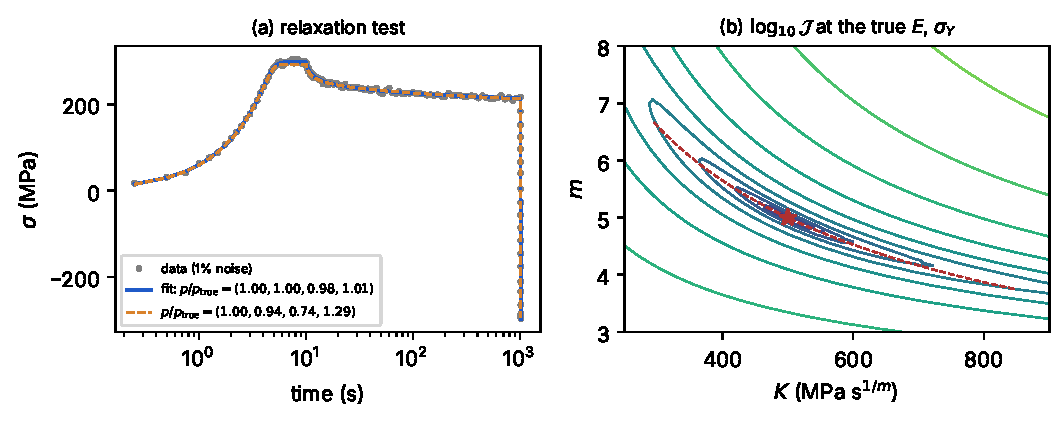
\includegraphics[width=0.92\textwidth]{figures/ch7/norton_id.pdf}
\caption{Norton--Hoff filament, relaxation test with a hold of $1000$\,s. (a)
Data with $1\%$ noise, the Levenberg--Marquardt fit, and the response of a
parameter set taken along the weakest Gauss--Newton direction: $K$ and $m$
change by $26\%$ and $29\%$, the stress by $2.9$\,MPa in the mean. (b) Level
lines of $\log_{10}\mathcal J$ in the plane $(K,m)$ at the true $E$ and $\sY$
(noise-free data); the star is the solution, the dashed line the weakest
direction of the $2\times2$ Gauss--Newton matrix.}
\label{fig:id-norton}
\end{figure}

%======================================================================
\section{Minimization algorithms}\label{sec:id-algo}
\index{minimization algorithms}%
This section presents the algorithms used in the chapter and compares them on
the truss; their principles, convergence properties and variants are collected
in Appendix~\ref{app:opt}, and \emph{Numerical Recipes}~\cite{PressEtAl2007b}
gives readable implementations of all of them.

\subsection{Without derivatives: the simplex of Nelder and Mead}
\index{Nelder--Mead method}%
The simplest algorithms use values of $\mathcal J$ only. The method of Nelder and
Mead~\cite{NelderMead1965} moves a simplex of $n_p+1$ points in the parameter
space. At each iteration the worst point is replaced by its reflection through
the centroid of the others, possibly expanded or contracted; if nothing works,
the simplex shrinks towards its best point.

\begin{gbox}{Box 7.1\quad Nelder--Mead simplex}
\index{Nelder--Mead method!Box 7.1}%
\begin{enumerate}[label=\textbf{\arabic*.},leftmargin=1.6em]
  \item \textbf{Order.} Sort the vertices, $\mathcal J(\vp_1)\le\dots\le\mathcal J(\vp_{n+1})$;
  $\bar\vp$ is the centroid of the $n$ best.
  \item \textbf{Reflect.} $\vp_r=\bar\vp+(\bar\vp-\vp_{n+1})$. If
  $\mathcal J(\vp_1)\le\mathcal J(\vp_r)<\mathcal J(\vp_n)$, replace $\vp_{n+1}$ by $\vp_r$.
  \item \textbf{Expand.} If $\mathcal J(\vp_r)<\mathcal J(\vp_1)$, try
  $\vp_e=\bar\vp+2(\bar\vp-\vp_{n+1})$ and keep the better of $\vp_e$, $\vp_r$.
  \item \textbf{Contract.} If $\mathcal J(\vp_r)\ge\mathcal J(\vp_n)$, try
  $\vp_c=\bar\vp+\tfrac12(\vp_{n+1}-\bar\vp)$ (or the outside contraction
  $\bar\vp+\tfrac12(\vp_r-\bar\vp)$); keep it if it improves on the worst point.
  \item \textbf{Shrink.} Otherwise, $\vp_i\gets\vp_1+\tfrac12(\vp_i-\vp_1)$ for all
  $i\ge2$.
  \item \textbf{Test.} Stop when the simplex and the spread of the values are small.
\end{enumerate}
\end{gbox}
The method needs no derivative, tolerates a noisy or non-smooth cost, and
costs one or two direct computations per iteration. Its weaknesses are as
clear. It has no convergence theory beyond small dimensions: Lagarias et
al.~\cite{LagariasEtAl1998} prove convergence for strictly convex functions in
one and two dimensions, and McKinnon~\cite{McKinnon1998} gives a strictly
convex function of two variables on which the simplex converges to a
non-stationary point. Its cost grows quickly with $n_p$, and it is easily
stopped by a curved valley. Genetic and evolutionary algorithms explore the
whole parameter space and find global minima, at the price of thousands of
direct computations~\cite{AndradeCamposEtAl2007}. They are useful to start
a gradient method, or when the direct computation is cheap.

\subsection{With derivatives}
\index{BFGS method}\index{Levenberg--Marquardt method}%
With the gradient, a descent method moves along $-\nabla\mathcal J$ or, better,
along a quasi-Newton direction. The BFGS method builds an approximation of the
Hessian from the successive gradients, and a line search along each direction
ensures a sufficient decrease~\cite{NocedalWright2006}. It needs one gradient per
iteration, which the adjoint method of Section~\ref{sec:id-grad} delivers at
the cost of about one more direct computation.

Least squares have more structure. The Gauss--Newton method minimizes the
quadratic model~\eqref{eq:id-GN} at each step,
$\mat{S}\T\mat{S}\,\delta\vp=-\mat{S}\T\mat{r}$, and needs the whole sensitivity
matrix. Levenberg and Marquardt add a damping that interpolates between
Gauss--Newton and steepest descent, and that makes the step safe far from the
solution and in flat valleys.

\begin{gbox}{Box 7.2\quad Levenberg--Marquardt}
\index{Levenberg--Marquardt method!Box 7.2}%
\begin{enumerate}[label=\textbf{\arabic*.},leftmargin=1.6em]
  \item \textbf{Direct problem and sensitivities.} At $\vp_k$, compute
  $\mat{r}(\vp_k)$ and $\mat{S}(\vp_k)$ (direct differentiation,
  Section~\ref{sec:id-path}).
  \item \textbf{Damped step.} Solve
  $(\mat{S}\T\mat{S}+\nu_k\,\mat{D})\,\delta\vp=-\mat{S}\T\mat{r}$, with $\mat{D}$ the
  diagonal of $\mat{S}\T\mat{S}$ (or $\mat{I}$).
  \item \textbf{Accept or reject.} If $\mathcal J(\vp_k+\delta\vp)<\mathcal J(\vp_k)$,
  accept the step and decrease $\nu$; otherwise increase $\nu$ and go back to 2.
  \item \textbf{Test.} Stop when $\norm{\mat{S}\T\mat{r}}$ or the step are small.
\end{enumerate}
\end{gbox}
\noindent Large $\nu$ gives a short step along the gradient; $\nu\to0$ gives
Gauss--Newton, which converges quadratically when the residual at the solution
vanishes, and linearly otherwise. Levenberg--Marquardt is the method of most
identification codes~\cite{MahnkenStein1996,LecampionConstantinescuNguyen2002}.

\paragraph{The truss.}
Figure~\ref{fig:id-truss} compares the three methods on the truss, in the
variables $\log\vp$, starting from $\vp_0=(0.7,1.2,3.0)\,\vp_{\mathrm{true}}$.
Levenberg--Marquardt with the sensitivities of the direct differentiation
reaches the minimum in 14 direct computations and 11 sensitivity computations;
BFGS with the adjoint gradient needs 28 direct and 28 adjoint computations. Both
find $\vp/\vp_{\mathrm{true}}=(1.0022,\,0.9992,\,1.0036)$, consistent with the
standard deviations of Section~\ref{ssec:id-sens}, and the cost
$\mathcal J=0.291$, below its value at the true parameters, $0.297$: the fit
cannot be better than the noise. The simplex stops after 1210 direct
computations at $(0.43,\,1.19,\,0)$, with the cost $453$: it has slid along the
valley of $(\sY,H)$ to the boundary $H=0$ and lost the minimum. From the start
$\vp_0=(0.7,1.5,3.0)\,\vp_{\mathrm{true}}$ the truss does not yield at all;
$\partial\mathcal J/\partial\sY$ and $\partial\mathcal J/\partial H$ vanish, and every
method adjusts $E$ alone, to the wrong value $0.44E$, which mimics the plastic
displacements by a softer elastic structure. The start must activate the
mechanisms that the parameters describe.

\begin{figure}[h]
\centering
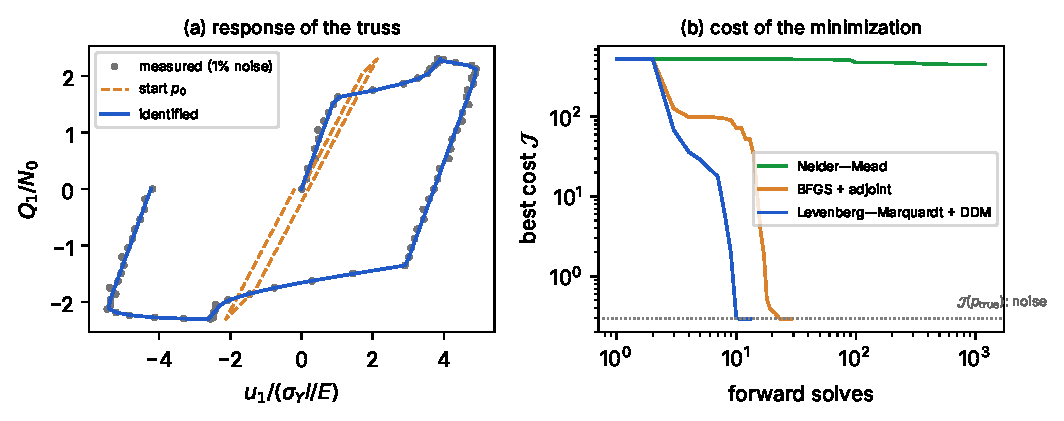
\includegraphics[width=0.92\textwidth]{figures/ch7/truss_id.pdf}
\caption{Identification of $(E,\sY,H)$ on the truss. (a) Measured response
$(u_1,Q_1)$, response at the start $\vp_0=(0.7,1.2,3.0)\,\vp_{\mathrm{true}}$ (the
dashed loops), and identified response. (b) Best cost against the number of
direct computations: Nelder--Mead, BFGS with the adjoint gradient (each
evaluation also costs one adjoint), Levenberg--Marquardt with the direct
differentiation (each Jacobian costs one sensitivity computation). The dotted
line is the cost at the true parameters.}
\label{fig:id-truss}
\end{figure}

\subsection{What a gradient costs}
\index{gradient!cost}%
A gradient-based method needs either the gradient $\nabla\mathcal J$ or the whole
matrix $\mat{S}$. The three ways of computing them, detailed in the next
sections, have very different costs (Table~\ref{tab:id-costs}).

\begin{table}[h]
\centering\small
\renewcommand{\arraystretch}{1.15}
\begin{tabular}{@{}llll@{}}
\toprule
\sffamily method & \sffamily delivers & \sffamily extra cost & \sffamily accuracy\\
\midrule
finite differences & $\mat{S}$ or $\nabla\mathcal J$ & $n_p$ (or $2n_p$) direct computations & $\sqrt{\epsilon}$, step to choose\\
direct differentiation & $\mat{S}$ & $n_p$ linear solves per step, forward & exact\\
adjoint state & $\nabla\mathcal J$ & one linear solve per step, backward & exact, history stored\\
\bottomrule
\end{tabular}
\caption{Cost of one gradient, beyond the direct computation; $n_p$ is the
number of parameters, $\epsilon$ the round-off level. The linear solves of the
two exact methods use the factorized tangent of the direct computation.}
\label{tab:id-costs}
\end{table}
\noindent Levenberg--Marquardt needs $\mat{S}$: direct differentiation is its
natural partner when $n_p$ is small. BFGS needs $\nabla\mathcal J$: the adjoint is
its natural partner when $n_p$ is large, a field of moduli, a distributed load,
the shape of a part. The two exact methods compute the derivative of the
discrete solution: they need no step and agree to round-off
(Section~\ref{sec:id-path}).

%======================================================================
\section{Three ways to compute a gradient}\label{sec:id-grad}
\index{gradient!computation}\index{sensitivity analysis}%
The three methods are first written for a linear problem in finite dimension,
the discrete elasticity problem of Chapter~\ref{ch:elliptic} with parameters
in the stiffness and in the loads:
\begin{equation}\label{eq:id-linear}
  \mat{K}(\vp)\,\mat{u}=\mat{f}(\vp),\qquad
  \mathcal J(\vp)=j\bigl(\mat{u}(\vp),\vp\bigr).
\end{equation}
The cost depends on $\vp$ directly and through the solution $\mat{u}(\vp)$.

\paragraph{Two springs.}
\index{springs!identification}%
Take the chain of Section~\ref{ssec:springs} with two springs, fixed at the
left end, loaded by a force $f$ at the right end. The stiffnesses $k_1$, $k_2$
are unknown and the displacement $u_2$ of the end is measured:
\[
  \mat{K}=\begin{bmatrix}k_1+k_2&-k_2\\-k_2&k_2\end{bmatrix},\qquad
  \mat{f}=\begin{bmatrix}0\\f\end{bmatrix},\qquad
  \mat{u}=f\begin{bmatrix}1/k_1\\1/k_1+1/k_2\end{bmatrix},\qquad
  \mathcal J=\tfrac12\,(u_2-u_2^m)^2 .
\]
The derivatives can be read on the solution: $\partial u_2/\partial k_1=-f/k_1^2$
and $\partial u_2/\partial k_2=-f/k_2^2$. One measurement gives one equation,
$1/k_1+1/k_2=u_2^m/f$: the two springs in series are seen through their total
compliance only. The sensitivity matrix $\mat{S}=-f\,[1/k_1^2,\ 1/k_2^2]$ has
rank one, and the Gauss--Newton matrix a zero eigenvalue. A second experiment,
a force on the middle node, gives $1/k_1$ alone and separates them
(Exercise~\ref{exo:id-q-springs}). The three methods below compute the same
derivatives without the closed form.

\subsection{Finite differences}\label{ssec:id-fd}
\index{finite differences}%
The forward difference
$\partial_j\mathcal J\approx(\mathcal J(\vp+h\ve_j)-\mathcal J(\vp))/h$ has a truncation error
$\tfrac12h\,|\partial^2_j\mathcal J|$ and a round-off error of order $\epsilon|\mathcal J|/h$,
where $\epsilon$ is the relative accuracy of the computed $\mathcal J$. Their sum is
smallest for $h\sim\sqrt{\epsilon}$, which leaves about half of the digits; the
central difference, with the truncation error $O(h^2)$, is best for
$h\sim\epsilon^{1/3}$. The accuracy $\epsilon$ is not the machine precision: it is
the tolerance of the Newton iterations, of the local returns, of the contact
algorithm. A tolerance of $10^{-6}$ limits the forward difference to three
digits. On the truss with a converged direct computation (Table~\ref{tab:id-fd}),
the relative steps from $10^{-2}$ to $10^{-10}$ show both errors. Each gradient
costs $n_p$ more direct computations, $2n_p$ for central differences.
Finite differences need nothing but the direct code, and remain the tool to
\emph{check} an exact gradient.

\subsection{Direct differentiation}\label{ssec:id-ddm}
\index{direct differentiation method}%
Differentiate~\eqref{eq:id-linear} with respect to $p_j$:
\begin{equation}\label{eq:id-ddm-lin}
  \mat{K}\,\frac{\partial\mat{u}}{\partial p_j}
  =\frac{\partial\mat{f}}{\partial p_j}-\frac{\partial\mat{K}}{\partial p_j}\,\mat{u},
  \qquad
  \frac{\dd\mathcal J}{\dd p_j}=\frac{\partial j}{\partial p_j}
  +\frac{\partial j}{\partial\mat{u}}\cdot\frac{\partial\mat{u}}{\partial p_j}.
\end{equation}
The sensitivity $\partial\mat{u}/\partial p_j$ solves the direct problem with the
same matrix and a \emph{pseudo-load}: the change of the loads minus the change
of the internal forces at fixed displacement. The factorization of $\mat{K}$ is
reused; each parameter costs one more right-hand side. The method gives the
whole matrix $\mat{S}$, and the sensitivity of every field, not only of the
observed ones. For the springs, $\partial\mat{K}/\partial k_1=\ve_1\ve_1\T$ and the
pseudo-load is $-u_1\ve_1$: a force $-f/k_1$ at the middle node, whose response
gives $\partial u_2/\partial k_1=-f/k_1^2$.

\subsection{The adjoint state}\label{ssec:id-adj}
\index{adjoint state}\index{Lagrangian!adjoint state}%
Adjoin the state equation to the cost with a multiplier $\boldsymbol\lambda$,
with the sign convention of Section~\ref{sec:var-lagrange}:
\begin{equation}\label{eq:id-lag-lin}
  \mathcal L(\mat{u},\boldsymbol\lambda,\vp)=j(\mat{u},\vp)-\boldsymbol\lambda\T\bigl(\mat{K}(\vp)\mat{u}-\mat{f}(\vp)\bigr).
\end{equation}
The three variables are independent. When $\mat{u}$ solves the state equation,
$\mathcal L=\mathcal J$ for every $\boldsymbol\lambda$. Choose $\boldsymbol\lambda$ so that
$\mathcal L$ does not depend on $\mat{u}$ to first order.
\begin{gbox}{The adjoint gives the whole gradient for one more solve}\label{prop:id-adj}
Let $\mat{u}$ solve $\mat{K}\mat{u}=\mat{f}$ and $\boldsymbol\lambda$ the \emph{adjoint problem}
\begin{equation}\label{eq:id-adj-lin}
  \mat{K}\T\boldsymbol\lambda=\frac{\partial j}{\partial\mat{u}} .
\end{equation}
Then, for all parameters at once,
\begin{equation}\label{eq:id-grad-lin}
  \frac{\dd\mathcal J}{\dd p_j}=\frac{\partial\mathcal L}{\partial p_j}
  =\frac{\partial j}{\partial p_j}
  -\boldsymbol\lambda\T\Bigl(\frac{\partial\mat{K}}{\partial p_j}\mat{u}-\frac{\partial\mat{f}}{\partial p_j}\Bigr).
\end{equation}
\end{gbox}
\paragraph{Why it works.} Insert~\eqref{eq:id-ddm-lin} in the derivative of the
cost: $\dd\mathcal J/\dd p_j=\partial_jj+(\partial_{\mat{u}}j)\T\mat{K}^{-1}(\partial_j\mat{f}-\partial_j\mat{K}\,\mat{u})$.
Group the product the other way:
$(\partial_{\mat{u}}j)\T\mat{K}^{-1}=(\mat{K}^{-\top}\partial_{\mat{u}}j)\T=\boldsymbol\lambda\T$.
The direct differentiation solves $n_p$ problems with $\mat{K}$; the adjoint
solves one problem with $\mat{K}\T$ and takes $n_p$ scalar products. The adjoint
answers the question: by how much does the cost change if a force $\delta\mat{f}$
is added to the structure? By $\boldsymbol\lambda\T\delta\mat{f}$. A parameter acts on
the structure as the pseudo-load $\partial_j\mat{f}-\partial_j\mat{K}\,\mat{u}$, and
its effect on the cost is the work of that pseudo-load in the adjoint
displacement. This is the reciprocity of Section~\ref{ssec:reciprocity},
used once more.

For the springs, $\partial j/\partial\mat{u}=(u_2-u_2^m)\ve_2$: the adjoint
structure is the same chain, loaded at the measured node by the misfit. Its
displacement is $\boldsymbol\lambda=(u_2-u_2^m)\,(1/k_1,\ 1/k_1+1/k_2)$, and the
gradient follows from two scalar products:
$\dd\mathcal J/\dd k_1=-\lambda_1u_1=-(u_2-u_2^m)f/k_1^2$ and
$\dd\mathcal J/\dd k_2=-(\lambda_2-\lambda_1)(u_2-u_1)=-(u_2-u_2^m)f/k_2^2$.

\paragraph{Continuous form.}
\index{adjoint state!elasticity}%
For the elastic body of Chapter~\ref{ch:elliptic} with the moduli
$\bbC(\vp)$ and the cost
$\displaystyle \mathcal J=\int_\Omega j_\Omega(\vu,\vp)\dd x+\int_{\partial\Omega}j_{\partial\Omega}(\vu,\vp)\dd s$,
the Lagrangian adjoins the weak form with a multiplier field $\vu^\star$, and
the same computation gives~\cite{BonnetConstantinescu2005}:
\begin{itemize}
  \item the \emph{adjoint problem} is an elasticity problem on the same body,
  with the body force $\partial j_\Omega/\partial\vu$ and the traction
  $\partial j_{\partial\Omega}/\partial\vu$: the misfits at the gauges act as forces;
  \item the \emph{gradient} is
  $\displaystyle \frac{\dd\mathcal J}{\dd p_j}=\frac{\partial\mathcal J}{\partial p_j}-\int_\Omega\eps[\vu]:\frac{\partial\bbC}{\partial p_j}:\eps[\vu^\star]\dd x$,
  plus the work of the derivatives of the loads in $\vu^\star$.
\end{itemize}
The gradient with respect to the modulus of an element is the product of the
direct and the adjoint strains in that element: the cost of the whole field of
gradients is one adjoint problem. This is why the adjoint is the method of
choice for distributed parameters and for shape optimization.

%======================================================================
\section{Contact: only the active constraints count}\label{sec:id-contact}
\index{contact!adjoint}\index{indentation!adjoint}\index{active set!adjoint}%
\subsection{The direct problem}
In the indentation problem the constraint $u\ge U-g$ holds on part of the
surface only, the contact zone, which is unknown. Discretized, the membrane of
Section~\ref{ssec:id-models} is a quadratic program
\begin{equation}\label{eq:id-contact}
  \min_{\mat{u}}\ \tfrac12\mat{u}\T\mat{K}\mat{u}
  \quad\text{s.t.}\quad \mat{u}\ge\mat{d},\qquad
  \mat{K}=k_f\mat{M}+T_m\mat{A},\quad d_i=U-g(x_i),
\end{equation}
with the lumped foundation matrix $\mat{M}$ and the membrane matrix $\mat{A}$.
With the multipliers $\mat{t}\ge\mat{0}$, the Lagrangian
$\tfrac12\mat{u}\T\mat{K}\mat{u}-\mat{t}\T(\mat{u}-\mat{d})$ gives the Kuhn--Tucker
conditions
\begin{equation}\label{eq:id-contact-kt}
  \mat{K}\mat{u}=\mat{t},\qquad \mat{t}\ge\mat{0},\qquad \mat{u}-\mat{d}\ge\mat{0},\qquad
  t_i\,(u_i-d_i)=0 ,
\end{equation}
and the multiplier is the contact force of the punch on the membrane; the
measured force is $F=\sum_it_i$ (Figure~\ref{fig:id-membrane}).

\begin{figure}[h]
\centering
\begin{tikzpicture}[>=Latex]
    % punch
    \fill[gray!25,domain=-0.43:0.43,samples=40] plot ({6*\x},{-12*(0.2-\x*\x)}) -- (2.58,1.3) -- (-2.58,1.3) -- cycle;
    \draw[thick,domain=-0.43:0.43,samples=40] plot ({6*\x},{-12*(0.2-\x*\x)});
    \draw[->,very thick,red!70!black] (0,1.3) -- (0,2.0) node[right,font=\small] {$F=\sum_it_i$};
    \node[font=\small] at (0,0.85) {rigid punch, $g(x)=x^2/(2R)$};
    % ground and supports
    \fill[pattern=north east lines] (-6.2,-3.55) rectangle (6.2,-3.4);
    \draw (-6.2,-3.4) -- (6.2,-3.4);
    \foreach \x in {-6,6}{\fill[pattern=north east lines] (\x-0.15,0) rectangle (\x+0.15,0.3);
       \draw[thick] (\x-0.15,0) -- (\x+0.15,0);}
    \draw[dashed,gray] (-6,0) -- (6,0);
    % springs and membrane
    \draw[spring,gray!65!black] (-5.400,-0.163) -- (-5.400,-3.4);
    \draw[spring,gray!65!black] (-4.800,-0.332) -- (-4.800,-3.4);
    \draw[spring,gray!65!black] (-4.200,-0.515) -- (-4.200,-3.4);
    \draw[spring,gray!65!black] (-3.600,-0.718) -- (-3.600,-3.4);
    \draw[spring,gray!65!black] (-3.000,-0.950) -- (-3.000,-3.4);
    \draw[spring,gray!65!black] (-2.400,-1.221) -- (-2.400,-3.4);
    \draw[spring,gray!65!black] (-1.800,-1.540) -- (-1.800,-3.4);
    \draw[spring,gray!65!black] (-1.200,-1.920) -- (-1.200,-3.4);
    \draw[spring,gray!65!black] (-0.600,-2.280) -- (-0.600,-3.4);
    \draw[spring,gray!65!black] (0.000,-2.400) -- (0.000,-3.4);
    \draw[spring,gray!65!black] (0.600,-2.280) -- (0.600,-3.4);
    \draw[spring,gray!65!black] (1.200,-1.920) -- (1.200,-3.4);
    \draw[spring,gray!65!black] (1.800,-1.540) -- (1.800,-3.4);
    \draw[spring,gray!65!black] (2.400,-1.221) -- (2.400,-3.4);
    \draw[spring,gray!65!black] (3.000,-0.950) -- (3.000,-3.4);
    \draw[spring,gray!65!black] (3.600,-0.718) -- (3.600,-3.4);
    \draw[spring,gray!65!black] (4.200,-0.515) -- (4.200,-3.4);
    \draw[spring,gray!65!black] (4.800,-0.332) -- (4.800,-3.4);
    \draw[spring,gray!65!black] (5.400,-0.163) -- (5.400,-3.4);
    \draw[very thick,cu] (-6.000,-0.000) -- (-5.400,-0.163) -- (-4.800,-0.332) -- (-4.200,-0.515) -- (-3.600,-0.718) -- (-3.000,-0.950) -- (-2.400,-1.221) -- (-1.800,-1.540) -- (-1.200,-1.920) -- (-0.600,-2.280) -- (0.000,-2.400) -- (0.600,-2.280) -- (1.200,-1.920) -- (1.800,-1.540) -- (2.400,-1.221) -- (3.000,-0.950) -- (3.600,-0.718) -- (4.200,-0.515) -- (4.800,-0.332) -- (5.400,-0.163) -- (6.000,-0.000);
    \draw[->,thick,red!70!black] (-1.200,-1.677) -- (-1.200,-1.870);
    \draw[->,thick,red!70!black] (-0.600,-1.452) -- (-0.600,-2.230);
    \draw[->,thick,red!70!black] (0.000,-1.560) -- (0.000,-2.350);
    \draw[->,thick,red!70!black] (0.600,-1.452) -- (0.600,-2.230);
    \draw[->,thick,red!70!black] (1.200,-1.677) -- (1.200,-1.870);
    \fill[white,draw=cu,thick] (-5.400,-0.163) circle (2pt);
    \fill[white,draw=cu,thick] (-4.800,-0.332) circle (2pt);
    \fill[white,draw=cu,thick] (-4.200,-0.515) circle (2pt);
    \fill[white,draw=cu,thick] (-3.600,-0.718) circle (2pt);
    \fill[white,draw=cu,thick] (-3.000,-0.950) circle (2pt);
    \fill[white,draw=cu,thick] (-2.400,-1.221) circle (2pt);
    \fill[white,draw=cu,thick] (-1.800,-1.540) circle (2pt);
    \fill[red!70!black] (-1.200,-1.920) circle (2.4pt);
    \fill[red!70!black] (-0.600,-2.280) circle (2.4pt);
    \fill[red!70!black] (0.000,-2.400) circle (2.4pt);
    \fill[red!70!black] (0.600,-2.280) circle (2.4pt);
    \fill[red!70!black] (1.200,-1.920) circle (2.4pt);
    \fill[white,draw=cu,thick] (1.800,-1.540) circle (2pt);
    \fill[white,draw=cu,thick] (2.400,-1.221) circle (2pt);
    \fill[white,draw=cu,thick] (3.000,-0.950) circle (2pt);
    \fill[white,draw=cu,thick] (3.600,-0.718) circle (2pt);
    \fill[white,draw=cu,thick] (4.200,-0.515) circle (2pt);
    \fill[white,draw=cu,thick] (4.800,-0.332) circle (2pt);
    \fill[white,draw=cu,thick] (5.400,-0.163) circle (2pt);
    % annotations
    \draw[dashed,gray] (6.15,0) -- (7.1,0);
    \draw[dashed,gray] (0.1,-2.4) -- (7.1,-2.4);
    \draw[<->,thick,cphi!80!black] (6.95,0) -- (6.95,-2.4) node[midway,right,font=\small,cphi!70!black] {$U$};
    \node[font=\small,cu,anchor=south west] at (-6.2,0.35) {membrane, tension $T_m$};
    \node[font=\small,gray!40!black,anchor=east] at (-6.3,-1.9) {foundation $k_f$};
    \draw[decorate,decoration={brace,amplitude=5pt,mirror},red!70!black] (-1.25,-3.7) -- (1.25,-3.7);
    \node[font=\small,red!70!black,anchor=north east] at (1.1,-3.95) {active set $\mathcal A$: $u_i=d_i$, $t_i\ge0$};
    \draw[decorate,decoration={brace,amplitude=5pt,mirror},cu] (1.6,-3.7) -- (5.5,-3.7)
      node[midway,below=5pt,font=\small,cu] {inactive set $\mathcal I$: $u_i>d_i$, $t_i=0$};
\end{tikzpicture}
\caption{The discrete indentation problem~\eqref{eq:id-contact}, drawn for 19
nodes, $(k_f,T_m)=(4,1)$, $R=0.5$, $U=0.2$ (deflections to scale). Each node
carries a spring of the foundation and is linked to its neighbours by the
membrane. On the active set (red) the node follows the punch, $u_i=d_i=U-g(x_i)$,
and the punch exerts the force $t_i\ge0$ (arrows); elsewhere the node is free and
$t_i=0$. The measured force is the sum of the contact forces.}
\label{fig:id-membrane}
\end{figure}
 These are the conditions of
Section~\ref{sec:var-lagrange} with inequalities, the same as the Kuhn--Tucker
conditions of plasticity. The nodes split into the \emph{active} set
$\mathcal A$, where $u_i=d_i$, and the inactive set $\mathcal I$, where $t_i=0$.
Once $\mathcal A$ is known the problem is linear: the membrane is clamped to the
punch on $\mathcal A$. The primal--dual active-set method finds $\mathcal A$ by
solving this linear problem, moving the nodes with a negative force out of
$\mathcal A$ and the penetrating nodes into it, and repeating; it is Newton's
method for the complementarity conditions.

\subsection{The adjoint problem}
Let $\mathcal J=\tfrac12(F(\vp)-F^m)^2$ at a given depth. Suppose that every
active node carries a strictly positive force and every inactive node a strictly
positive gap: \emph{strict complementarity}. A small change of $\vp$ then keeps
the active set, and the solution is that of the linear problem
\begin{equation}\label{eq:id-contact-lin}
  \mat{K}(\vp)\mat{u}=\mat{t},\qquad u_i=d_i\ (i\in\mathcal A),\qquad t_i=0\ (i\in\mathcal I),
\end{equation}
whose data $d_i$ do not depend on $\vp$. Its derivative is that of a problem with
\emph{imposed displacements} on the contact zone.

\begin{gbox}{The adjoint of a contact problem is not a contact problem}\label{prop:id-contact}
Under strict complementarity, let $\mat{v}$ be the elastic solution with the
imposed displacements $v_i=F-F^m$ on the active set $\mathcal A$ of the direct
solution and no force elsewhere:
\begin{equation}\label{eq:id-contact-adj}
  (\mat{K}\mat{v})_i=0\ \ (i\in\mathcal I),\qquad v_i=F-F^m\ \ (i\in\mathcal A).
\end{equation}
Then
\begin{equation}\label{eq:id-contact-grad}
  \frac{\dd\mathcal J}{\dd p_j}=\mat{v}\T\,\frac{\partial\mat{K}}{\partial p_j}\,\mat{u}
  \qquad\Bigl(\text{continuous form: }
  \int_\Omega\eps[\vu]:\frac{\partial\bbC}{\partial p_j}:\eps[\vv]\dd x\Bigr).
\end{equation}
The adjoint problem is linear, with Dirichlet data on the contact zone found by
the direct computation; the inactive constraints do not appear.
\end{gbox}
\paragraph{Why it works.} Freeze the active set and differentiate~\eqref{eq:id-contact-lin}:
$\delta u_i=0$ on $\mathcal A$, $\delta t_i=0$ on $\mathcal I$, and
$\mat{K}\,\delta\mat{u}+\delta\mat{K}\,\mat{u}=\delta\mat{t}$. Let $\hat{\mat{v}}$ be the
field~\eqref{eq:id-contact-adj} with the unit datum $\hat v_i=1$ on $\mathcal A$.
Multiply the differentiated equation by $\hat{\mat{v}}$ and use the symmetry of $\mat{K}$:
$\hat{\mat{v}}\T\mat{K}\delta\mat{u}=(\mat{K}\hat{\mat{v}})\T\delta\mat{u}=0$, because
$\mat{K}\hat{\mat{v}}$ vanishes on $\mathcal I$ and $\delta\mat{u}$ vanishes on $\mathcal A$.
What remains is $\hat{\mat{v}}\T\delta\mat{K}\,\mat{u}=\hat{\mat{v}}\T\delta\mat{t}=\sum_{i\in\mathcal A}\delta t_i=\delta F$.
The derivative of the force is the reciprocal work of the change of stiffness
between the direct field and the field of a unit settlement of the contact zone;
multiply by $F-F^m$. In the language of Lagrangians: the multiplier of the
constraint $u_i=d_i$ on the active set is free, the one of an inactive node is
zero, and the stationarity with respect to the forces $t_i$ imposes the value of
the adjoint displacement on $\mathcal A$.

Tardieu and Constantinescu~\cite{TardieuConstantinescu2000} obtained this
result for the Signorini problem of an elastic body indented by a rigid punch,
by two routes: the penalized formulation, whose adjoint is an elastic problem
with springs of stiffness $1/\epsilon$ on the penetrated zone, which become a
Dirichlet condition as $\epsilon\to0$; and the mixed formulation, in which the
adjoint multiplier is sought in the space of pressures that vanish outside the
effective contact zone, not in the cone of positive pressures. Choosing the
cone would turn the stationarity conditions into coupled variational
inequalities; choosing the space of the active zone gives a linear problem. The
gradient~\eqref{eq:id-contact-grad} agreed with finite differences to four or
five digits on their axisymmetric indentation by a cone (for instance $-10.383$
against $-10.380$), and identified the two moduli of a coated body to $0.001\%$.

\paragraph{The membrane.}
Table~\ref{tab:id-contact} compares~\eqref{eq:id-contact-grad} with central
differences on the membrane: they agree to all the printed digits, at shallow and
deep indentation. Figure~\ref{fig:id-indent}a shows the adjoint field: it is
the membrane lifted by a unit displacement of the contact zone, decaying to the
fixed ends with the length $\sqrt{T_m/k_f}$.

\begin{table}[h]
\centering\small
\renewcommand{\arraystretch}{1.15}
\begin{tabular}{@{}ccccccc@{}}
\toprule
$U$ & $(k_f,T_m)$ & $F$ & $\partial F/\partial k_f$ (adjoint) & (FD) & $\partial F/\partial T_m$ (adjoint) & (FD)\\
\midrule
0.02 & (4, 1) & 0.0847 & 0.009488 & 0.009488 & 0.046715 & 0.046715\\
0.20 & (4, 1) & 0.9952 & 0.135419 & 0.135419 & 0.453522 & 0.453522\\
0.20 & (2, 3) & 1.5698 & 0.149455 & 0.149455 & 0.423646 & 0.423646\\
0.10 & (6, 0.5) & 0.4365 & 0.049544 & 0.049544 & 0.278532 & 0.278532\\
\bottomrule
\end{tabular}
\caption{Membrane indented by a parabolic punch, 79 nodes: derivative of the
force by the adjoint~\eqref{eq:id-contact-grad} and by central differences
(relative step $10^{-6}$). The contact zones have 3, 15, 11 and 13 nodes
(Exercise~\ref{exo:id-indent}).}
\label{tab:id-contact}
\end{table}

\begin{figure}[h]
\centering
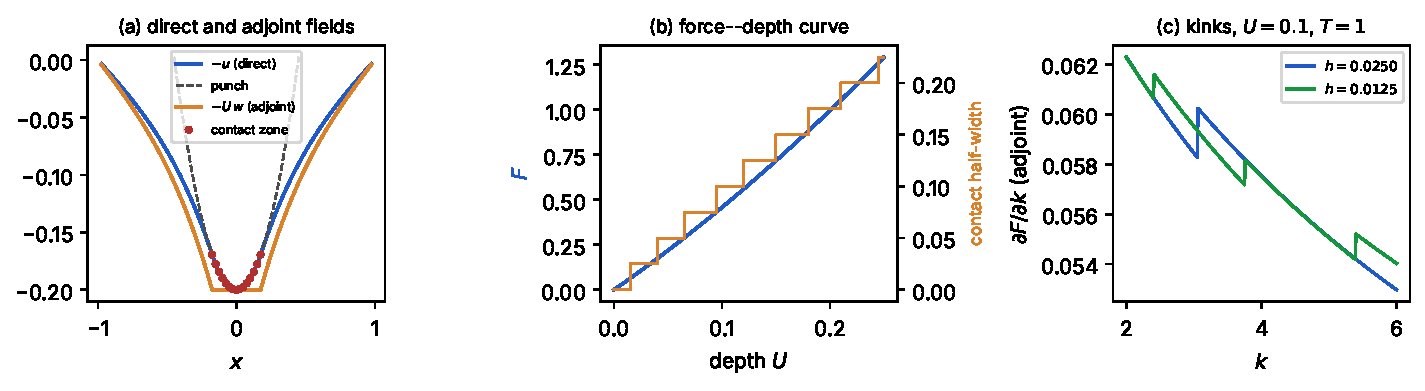
\includegraphics[width=\textwidth]{figures/ch7/indentation.pdf}
\caption{The membrane on an elastic foundation, $(k_f,T_m)=(4,1)$. (a) At the
depth $U=0.2$: deflection (blue), punch (dashed), contact zone (red dots), and
adjoint field $\hat v$ of~\eqref{eq:id-contact-adj} with a unit datum, scaled by
$U$ (orange). (b) Force and half-width of the contact zone against the depth:
the zone grows node by node. (c) $\partial F/\partial k_f$ at $U=0.1$ as a
function of $k_f$, for two meshes: the derivative jumps when a node enters the
contact zone; the jumps shrink with the mesh size.}
\label{fig:id-indent}
\end{figure}

\subsection{Kinks}\label{ssec:id-kinks}
\index{kinks!active set}\index{biactive constraint}%
What happens when strict complementarity fails? At a parameter value where a
node of the boundary of the contact zone has both a zero gap and a zero force,
the node is \emph{biactive}: it is about to enter or leave the contact zone. On
one side the active set contains it, on the other side not, and the two linear
problems~\eqref{eq:id-contact-lin} give two different derivatives. The force is
continuous but has a kink. Figure~\ref{fig:id-indent}c shows the jumps of
$\partial F/\partial k_f$ on the membrane: $3.4\%$, $1.9\%$ and $0.9\%$ of the derivative
for the mesh sizes $0.025$, $0.0125$ and $0.0063$. Each jump is the contribution
of one node, and it decreases with the mesh size; the continuous problem shows
no kink in this example, as Tardieu and Constantinescu observed for indentation.
The derivative with respect to the parameters of the contact itself, a gap or
the shape of the punch, is another matter: Hilding, Klarbring and
Petersson~\cite{HildingKlarbringPetersson1999} show that it may genuinely fail
to exist.

\paragraph{Identification.}
\index{indentation!identification}%
The two parameters are identified from the forces at two depths, $U=0.02$ and
$U=0.2$, with Levenberg--Marquardt and the adjoint derivatives. From the four
starts $(0.2,0.2)$, $(0.2,5)$, $(5,0.2)$, $(5,5)\times(k_f,T_m)_{\mathrm{true}}$ the
method returns the true values in 8 to 23 iterations. The relative sensitivities
$\partial\log F/\partial\log(k_f,T_m)$ are $(0.448,0.552)$ at the shallow depth and
$(0.544,0.456)$ at the deep one; at each depth they add up to one, the
homogeneity of Section~\ref{ssec:id-tell}. The shallow depth sees the membrane
a little more, the deep one the foundation: the information that separates the
two parameters is the difference of these two rows, which is why both depths
are needed. In the same way, Tardieu and Constantinescu separate the moduli of a
coating and of its substrate with a shallow and a deep indentation, each cost
being sensitive mainly to one of them~\cite{TardieuConstantinescu2000}.

\paragraph{The same structure in plasticity.}
\index{active set!plasticity}%
The return map of Chapter~\ref{ch:pl-num} solves, at each Gauss point, the
Kuhn--Tucker conditions $\dg\ge0$, $f\le0$, $\dg f=0$. A plastic point is an
active constraint, an elastic point an inactive one, and a point exactly at yield
with no flow, $f^\trial=0$, is biactive. The next section shows that the
derivative of the return map is the derivative of the active branch, and that
biactive points produce kinks, exactly as in contact.

%======================================================================
\section{Path-dependent problems: differentiating the incremental chain}\label{sec:id-path}
\index{sensitivity analysis!path-dependent}\index{adjoint state!elastoplasticity}%
\subsection{The incremental chain}
The elastoplastic computation of Chapter~\ref{ch:pl-num} is a chain of steps,
and its unknowns live in two places. The displacements $\mat{u}_n$ and the
forces $\mat{F}_n$ are nodal: equilibrium is written at the nodes. The strain, the
stress and the internal variables $\vz_n$ are stored at the Gauss points: the
strain $\eps_n=\mat{B}\mat{u}_n$ at a Gauss point is computed from the nodal
displacements of its element, and the return map gives there the stress and the
new internal variables from those of the previous step. At the step $n$:
\begin{equation}\label{eq:id-chain}
\begin{aligned}
  &\mat{R}_n:=\sum_e\int_{\Omega_e}\mat{B}\T\sig_n\dd x-\mat{F}_n=\mat{0}
  &&\text{(at the nodes)},\\
  &\eps_n=\mat{B}\mat{u}_n,\quad
  \sig_n=\hat\sig(\eps_n,\vz_{n-1};\vp),\quad
  \vz_n=\hat\vz(\eps_n,\vz_{n-1};\vp)
  &&\text{(at each Gauss point)},
\end{aligned}
\end{equation}
where $(\hat\sig,\hat\vz)$ is the return map $\mathcal R$ of~\eqref{eq:pn-returnmap},
now with the parameters written explicitly. The cost collects the observations
of all the steps, $\mathcal J=\sum_nj_n(\mat{u}_n)$. A change of the parameters acts on
every step directly, and on the later steps through the internal variables it
leaves behind. Differentiating the chain therefore needs the derivatives of the
return map with respect to its three arguments, at the converged state:
\[
  \bbCalg_n=\frac{\partial\hat\sig}{\partial\eps},\quad
  \hat\sig_{,\vz}=\frac{\partial\hat\sig}{\partial\vz_{n-1}},\quad
  \hat\sig_{,\vp}=\frac{\partial\hat\sig}{\partial\vp},\qquad
  \hat\vz_{,\eps},\quad\hat\vz_{,\vz},\quad\hat\vz_{,\vp}\ \ \text{likewise}.
\]
The first is the consistent tangent of Section~\ref{ssec:pn-calg}; the others are
computed in the same way, by differentiating the equations of the return map.

\paragraph{The filament.}
\index{return map!derivatives}%
Take Box~5.1 with linear kinematic hardening ($K=0$) and $\vp=(E,\sY,H)$. In an
elastic step the plastic strain is copied and the stress is linear:
\[
  \hat\sigma_{,\varepsilon}=E,\quad \hat\sigma_{,z}=-E,\quad
  \hat\sigma_{,\vp}=(\varepsilon-\varepsilon^p_{n-1},\,0,\,0),\qquad
  \hat z_{,\varepsilon}=0,\quad \hat z_{,z}=1,\quad \hat z_{,\vp}=\vzero .
\]
In a plastic step the end state lies on the yield surface,
$E(\varepsilon-\varepsilon^p_n)-H\varepsilon^p_n=s\,\sY$ with $s=\pm1$, hence
$\varepsilon^p_n=(E\varepsilon-s\sY)/(E+H)$: the new plastic strain no longer depends
on the old one, and
\[
  \hat\sigma_{,\varepsilon}=\frac{EH}{E+H},\quad \hat\sigma_{,z}=0,\quad
  \hat\sigma_{,\sY}=\frac{sE}{E+H},\qquad
  \hat z_{,\varepsilon}=\frac{E}{E+H},\quad \hat z_{,z}=0,\quad
  \hat z_{,\sY}=-\frac{s}{E+H} .
\]
The two sets of formulas are the derivatives of two different linear maps: the
elastic branch and the plastic branch. The derivative of the return map is
the derivative of the branch that is active.

\begin{gbox}{The derivative of the return map freezes the active set}\label{prop:id-rm}
At a point where the trial function $f^\trial\ne0$, the return map is
differentiable, and its derivatives are those of the elastic update ($f^\trial<0$)
or of the plastic update with the plastic multiplier determined by $f=0$
($f^\trial>0$). At a point where $f^\trial=0$, the point is at yield without
flowing, the two branches meet, and the return map has a kink: its
directional derivatives exist but differ.
\end{gbox}
\paragraph{Why it works.} In the filament, $\dg=\mac{f^\trial}/(E+K+H)$ is a ramp
function of the trial value. Away from zero the ramp is either $0$ or linear,
and differentiable; at zero it has a corner. For $J_2$ plasticity the same holds
with the radial return: the multiplier solves $g(\dg)=0$, and the implicit
function theorem gives its derivative as long as the step is plastic. A biactive
point, at yield with $\dg=0$, is the corner. One step of the filament shows the
jump: at fixed strain, $\partial\sigma/\partial\sY$ is $E/(E+H)$ when the step is
plastic and $0$ when it is elastic (Exercise~\ref{exo:id-q-kink}).

\subsection{Direct differentiation}\label{ssec:id-path-ddm}
\index{direct differentiation method!elastoplasticity}%
Differentiate~\eqref{eq:id-chain} with respect to $\vp$, along the chain.
Write $\delta(\cdot)=\partial(\cdot)/\partial p_j$ for one parameter.
Which matrix multiplies the unknown sensitivity $\delta\mat{u}_n$? The answer
decides the cost of both exact methods.

\begin{gbox}{The consistent tangent at the converged state is the operator of both exact methods}\label{prop:id-ctan}
The sensitivity problem of step $n$ has the matrix
$\mat{K}^{\mathrm{alg}}_n=\sum_e\int\mat{B}\T\bbCalg_n\mat{B}\dd x$, the consistent
tangent of the return map evaluated at the \emph{converged} state
$(\mat{u}_n,\vz_{n-1})$ of the step; the adjoint problem of step $n$ has its
transpose. Neither the continuum tangent $\bbCep$, nor the matrix of an
intermediate Newton iteration, nor the elastic stiffness of a modified Newton
method gives the exact derivative.
\end{gbox}
\paragraph{Why it works.} The converged step satisfies the nodal equations
$\mat{R}_n\bigl(\mat{u}_n(\vp),\vz_{n-1}(\vp);\vp\bigr)=\mat{0}$ for every $\vp$, with
$\sig_n=\hat\sig(\mat{B}\mat{u}_n,\vz_{n-1};\vp)$ at the Gauss points. Differentiate
this identity: the implicit function theorem gives
$\dfrac{\partial\mat{R}_n}{\partial\mat{u}_n}\,\delta\mat{u}_n
=-\dfrac{\partial\mat{R}_n}{\partial\vz_{n-1}}\,\delta\vz_{n-1}-\dfrac{\partial\mat{R}_n}{\partial p_j}$,
and $\partial\mat{R}_n/\partial\mat{u}_n=\sum_e\int\mat{B}\T(\partial\hat\sig/\partial\eps)\mat{B}$,
where $\partial\hat\sig/\partial\eps$ is the derivative of the return map that the
code actually runs, at the strain where it converged: the consistent tangent of
Section~\ref{ssec:pn-calg}, by definition. Three consequences follow.
\begin{itemize}
  \item The way the step was converged does not matter: the derivative of the
  solution does not depend on the path of the iterations. A forward solver that
  used Newton with the consistent tangent has the matrix ready, provided it is
  evaluated at the converged state (one more assembly if the last iteration
  updated the state after the last factorization). A solver that used the elastic
  stiffness (Box~6.1) or a quasi-Newton update must assemble and factorize
  $\mat{K}^{\mathrm{alg}}_n$ once at convergence, or solve with it iteratively.
  \item The tangent must be \emph{consistent} with the time discretization. The
  continuum tangent $\bbCep$ is the derivative of the rate equations, not of the
  discrete update: with it the sensitivities are wrong by a term of the order of
  the step size, and the gradient is not the gradient of the computed cost; Vidal,
  Lee and Haber~\cite{VidalLeeHaber1991} made this point.
  \item The adjoint differentiates the same identity with respect to $\mat{u}_n$
  inside the Lagrangian~\eqref{eq:id-lag-path} and meets
  $(\partial\mat{R}_n/\partial\mat{u}_n)\T=(\mat{K}^{\mathrm{alg}}_n)\T$. For associated
  plasticity the consistent tangent of the closest-point projection is symmetric
  (Section~\ref{ssec:pn-calg}), and the adjoint reuses the same factorization; a
  non-associated law gives a non-symmetric tangent and a transposed solve.
\end{itemize}

\begin{gbox}{Box 7.3\quad Direct differentiation of an elastoplastic computation}
\index{direct differentiation method!Box 7.3}%
\begin{enumerate}[label=\textbf{\arabic*.},leftmargin=1.6em]
  \item \textbf{Initialization.} $\delta\vz_0=\partial\vz_0/\partial p_j$ (usually
  zero) at each Gauss point.
  \item \textbf{Step $n$, after convergence of the direct step.} Assemble (or
  reuse) the consistent tangent at the converged state,
  $\mat{K}^{\mathrm{alg}}_n=\sum_e\int\mat{B}\T\bbCalg_n\mat{B}$ with $\bbCalg_n$ evaluated
  at $(\eps_n,\vz_{n-1})$, and solve
  \[
    \mat{K}^{\mathrm{alg}}_n\,\delta\mat{u}_n=\delta\mat{F}_n
    -\sum_e\int_{\Omega_e}\mat{B}\T\bigl(\hat\sig_{,\vz}\,\delta\vz_{n-1}+\hat\sig_{,p_j}\bigr)\dd x .
  \]
  \item \textbf{Local update.} At each Gauss point, with the strain sensitivity
  $\mat{B}\delta\mat{u}_n$ computed from the nodal values of the element,
  $\delta\vz_n=\hat\vz_{,\eps}\,\mat{B}\delta\mat{u}_n+\hat\vz_{,\vz}\,\delta\vz_{n-1}+\hat\vz_{,p_j}$.
  \item \textbf{Observations.} $\partial\mat{y}_n/\partial p_j$ from $\delta\mat{u}_n$;
  next step.
\end{enumerate}
\end{gbox}
\noindent The sensitivity problem is linear and marches forward with the direct
computation (Figure~\ref{fig:id-sweeps}). Its matrix is the consistent tangent of
the converged step (Section~\ref{prop:id-ctan}), factorized once per step and
shared by all the parameters: each parameter costs one more right-hand side per
step. Its
loads are the history terms $\hat\sig_{,\vz}\delta\vz_{n-1}$ and the explicit
dependence $\hat\sig_{,p_j}$. Vidal, Lee and Haber~\cite{VidalLeeHaber1991}
showed that the consistent tangent is the operator of the sensitivity problem;
Vidal and Haber~\cite{VidalHaber1993} wrote the method for rate-independent
elastoplasticity, and Kleiber et al.~\cite{KleiberEtAl1997} and Mahnken and
Stein~\cite{MahnkenStein1996} used it for identification.

\paragraph{Viscoplasticity.}
\index{direct differentiation method!viscoplasticity}%
For a Perzyna or Norton--Hoff material, the backward Euler update
$\eps^{vp}_n=\eps^{vp}_{n-1}+\Delta t\,\partial_{\sig}\varphi^\ast(\sig_n;\vp)$ is
differentiated in the same way. Eliminating $\delta\eps^{vp}_n$ gives
\[
  \delta\sig_n=\boldsymbol\Xi_n:\Bigl[\eps[\delta\vu_n]-\delta\eps^{vp}_{n-1}
  -\Delta t\,\frac{\partial^2\varphi^\ast}{\partial\sig\,\partial p_j}
  +\bbC^{-1}:\frac{\partial\bbC}{\partial p_j}:(\eps_n-\eps^{vp}_n)\Bigr],\qquad
  \boldsymbol\Xi_n=\Bigl(\bbS+\Delta t\,\frac{\partial^2\varphi^\ast}{\partial\sig^2}\Bigr)^{-1},
\]
with the consistent tangent $\boldsymbol\Xi_n$ of the viscoplastic return. The
sensitivity law is a linear viscoelastic law: the stress sensitivity depends on
the strain sensitivity of the step and on the sensitivities stored at the
previous step. Lecampion et al.~\cite{LecampionConstantinescuNguyen2002}
programmed it in Cast3M for a lined tunnel in a Norton--Hoff rock: the four
sensitivities cost about half of the direct computation, and they show where
and when each parameter matters, the viscoplastic zone around the tunnel and the
first years after the excavation. The sensitivities of the Norton filament of
this chapter are computed in the same way, by differentiating its scalar return
equation (Exercise~\ref{exo:id-norton}).

\subsection{The adjoint state}\label{ssec:id-path-adj}
\index{adjoint state!backward in time}%
Adjoin the equations of every step to the cost: the nodal equilibrium
equations with nodal multipliers $\boldsymbol\lambda_n$, an adjoint displacement
with one value per nodal degree of freedom, and the update of the internal
variables with multipliers $\boldsymbol\mu_n$ stored, like $\vz_n$, at the Gauss
points. At a Gauss point, $\mat{B}\boldsymbol\lambda_n$ is the adjoint strain:
\begin{equation}\label{eq:id-lag-path}
  \mathcal L=\sum_{n=1}^Nj_n(\mat{u}_n)-\sum_{n=1}^N\boldsymbol\lambda_n\T\mat{R}_n
  -\sum_{n=1}^N\int_\Omega\boldsymbol\mu_n\cdot\bigl(\vz_n-\hat\vz(\eps_n,\vz_{n-1};\vp)\bigr)\dd x .
\end{equation}
The internal variable $\vz_n$ appears in two steps: as the result of step $n$
and as the history of step $n+1$. Its stationarity therefore links the
multipliers of two successive steps, and the recursion runs from the end.

\begin{gbox}{Box 7.4\quad Adjoint of an elastoplastic computation}
\index{adjoint state!Box 7.4}%
\begin{enumerate}[label=\textbf{\arabic*.},leftmargin=1.6em]
  \item \textbf{Direct computation.} Run Box~5.3 and store the converged states:
  the nodal displacements $\mat{u}_n$ and the internal variables $\vz_n$ at the
  Gauss points (or only checkpoints, Section~\ref{ssec:id-storage}).
  \item \textbf{Terminal condition.} $\boldsymbol\mu_N=\vzero$: nothing follows the
  last step.
  \item \textbf{Step $n=N,\dots,1$, backward.} Recompute at each Gauss point the
  return map at the converged state $(\eps_n,\vz_{n-1})$, its consistent tangent
  $\bbCalg_n$ and the derivatives $\hat\sig_{,\vz}$, $\hat\sig_{,\vp}$, $\hat\vz_{,\eps}$,
  $\hat\vz_{,\vz}$, $\hat\vz_{,\vp}$; assemble $\mat{K}^{\mathrm{alg}}_n$ and solve the
  adjoint equilibrium, at the nodes, with its transpose,
  \[
    (\mat{K}^{\mathrm{alg}}_n)\T\boldsymbol\lambda_n=\frac{\partial j_n}{\partial\mat{u}_n}
    +\sum_e\int_{\Omega_e}\mat{B}\T\hat\vz_{,\eps}\T\boldsymbol\mu_n\dd x .
  \]
  \item \textbf{Gradient.} Add the contribution of the step,
  \[
    \nabla\mathcal J\mathrel{+}=-\int_\Omega\hat\sig_{,\vp}\T\,\mat{B}\boldsymbol\lambda_n\dd x
    +\int_\Omega\hat\vz_{,\vp}\T\boldsymbol\mu_n\dd x .
  \]
  \item \textbf{Local adjoint update.} At each Gauss point, with the adjoint strain
  $\mat{B}\boldsymbol\lambda_n$ computed from the nodal values of the element,
  $\boldsymbol\mu_{n-1}=\hat\vz_{,\vz}\T\boldsymbol\mu_n-\hat\sig_{,\vz}\T\,\mat{B}\boldsymbol\lambda_n$.
\end{enumerate}
\end{gbox}

\begin{gbox}{The adjoint of an evolution runs backward in time}\label{prop:id-backward}
The gradient of a cost of an elastoplastic evolution is obtained from the direct
computation and one backward sweep, Box~7.4, whatever the number of parameters.
Each backward step is a linear problem with the transposed consistent tangent of
the corresponding direct step; the adjoint sees the active set of the direct
computation, step by step. The local multiplier $\boldsymbol\mu$ carries the memory
of the material backward, from the observations to the instants that produced
them.
\end{gbox}
\paragraph{Why it works.} Write the stationarity of~\eqref{eq:id-lag-path}. With
respect to $\mat{u}_n$, which appears only in step $n$, it is the adjoint
equilibrium of step~3. With respect to $\vz_{n-1}$, which appears as the result
of step $n-1$ and as the history of step $n$, it is
$-\boldsymbol\mu_{n-1}-\hat\sig_{,\vz}\T\mat{B}\boldsymbol\lambda_n+\hat\vz_{,\vz}\T\boldsymbol\mu_n=\vzero$:
step~5. With respect to $\vz_N$, which has no successor, it is
$\boldsymbol\mu_N=\vzero$. When these hold and the direct equations are satisfied,
$\mathcal L=\mathcal J$ and $\dd\mathcal J/\dd\vp=\partial\mathcal L/\partial\vp$, which is
step~4. The order of the computation follows from the structure: step~5 needs
$\boldsymbol\lambda_n$, step~3 needs $\boldsymbol\mu_n$, and $\boldsymbol\mu_N$ is the only
one known. Michaleris, Tortorelli and Vidal~\cite{MichalerisTortorelliVidal1994}
derived both the direct and the adjoint sensitivities of transient coupled
problems from the consistent tangents in this way, and Tsay and
Arora~\cite{TsayArora1990} earlier for path-dependent structures.

\paragraph{The memory of the filament.}
For the filament, step~5 reads $\mu_{n-1}=\mu_n+E\,(\mat{B}\boldsymbol\lambda_n)$ in an
elastic step and $\mu_{n-1}=0$ in a plastic step. A plastic step of a material
with linear kinematic hardening forgets its history, since $\varepsilon^p_n$ does
not depend on $\varepsilon^p_{n-1}$; the adjoint memory is reset accordingly. An
elastic step carries the plastic strain unchanged, and the adjoint carries the
sensitivity to it backward, through the stress. This is the reversed image of
Chapter~\ref{ch:pl-cyc}, where an error made at a plastic instant is carried
unchanged by the elastic steps that follow.

\paragraph{The truss.}
Table~\ref{tab:id-fd} computes the gradient of the cost of the truss three ways,
at $\vp=(0.9,1.2,1.5)\,\vp_{\mathrm{true}}$, with the direct computation converged to
$10^{-13}$. The direct differentiation (Box~7.3) and the adjoint (Box~7.4) agree
with each other to all digits and with the central difference to eight digits.
The forward difference shows its two errors: truncation for large steps, round-off
for small ones, with the best accuracy, seven digits, near the relative step
$10^{-8}=\sqrt{\epsilon}$.

\begin{table}[h]
\centering\small
\renewcommand{\arraystretch}{1.15}
\begin{tabular}{@{}lccc@{}}
\toprule
\sffamily method & $E\,\partial\mathcal J/\partial E$ & $\sY\,\partial\mathcal J/\partial\sY$ & $H\,\partial\mathcal J/\partial H$\\
\midrule
forward difference, $h=10^{-2}$ & 178.895 & 303.257 & 5.95744\\
forward difference, $h=10^{-4}$ & 179.796 & 305.786 & 5.96701\\
forward difference, $h=10^{-6}$ & 179.8054 & 305.7776 & 5.967106\\
forward difference, $h=10^{-8}$ & 179.80547 & 305.77755 & 5.967104\\
forward difference, $h=10^{-10}$ & 179.8071 & 305.7778 & 5.96970\\
central difference, $h=10^{-6}$ & 179.805452 & 305.777548 & 5.967107\\
direct differentiation (Box~7.3) & 179.805452 & 305.777548 & 5.967107\\
adjoint (Box~7.4) & 179.805452 & 305.777548 & 5.967107\\
\bottomrule
\end{tabular}
\caption{Gradient of the cost of the truss with respect to $\log\vp$ at
$\vp=(0.9,1.2,1.5)\,\vp_{\mathrm{true}}$; $h$ is the relative step
(Exercise~\ref{exo:id-truss}).}
\label{tab:id-fd}
\end{table}

\subsection{What the adjoint must store}\label{ssec:id-storage}
\index{checkpointing}\index{adjoint state!storage}%
The backward sweep visits the steps in reverse order, and at each step it needs
the consistent tangent and the derivatives of the return map at the converged
state of that step. How much of the forward computation must be kept?

\paragraph{States, not matrices.}
Everything the backward step needs is a function of the converged state
$(\mat{u}_n,\vz_{n-1})$ and of $\vp$: the tangent and the derivatives are recomputed
by one call of the return map at each Gauss point, an assembly and a
factorization (Box~7.4, step~3). Storing the factorized tangents is never
worth it: a factorized stiffness matrix is far larger than a state. For a model
with $10^5$ nodes and $10^6$ Gauss points carrying 13 internal variables (plastic
strain, back stress, cumulated plastic strain), a state is about $1.3\times10^7$
numbers, $100$\,MB; a thousand steps make $100$\,GB. The states themselves may
already be too many.

\paragraph{Checkpoints and recomputation.}
Keep the state only at every $c$-th step, the \emph{checkpoints}. In the backward
sweep, recompute the steps of each segment from its checkpoint, forward and with
Newton, store their states, and run the adjoint through the segment. The gradient
is exact, the extra cost is one more forward sweep, and the memory is the
$N/c$ checkpoints plus one segment of $c$ states, smallest, about $2\sqrt N$,
for $c\approx\sqrt N$. Recursive (binomial) checkpointing does better: with $s$
checkpoints and at most $r$ recomputations of each step, it reverses
$\binom{s+r}{s}$ steps, so that memory and recomputation grow only
logarithmically with the number of steps~\cite{GriewankWalther2008}.

\paragraph{Interpolation?}
Can one skip the recomputation and interpolate the states between the
checkpoints? On the truss (Table~\ref{tab:id-storage}, Figure~\ref{fig:id-storage}),
linear interpolation in time gives a gradient error of $0.07\%$ with a checkpoint
every second step, $1\%$ every fourth or fifth, $6\%$ every tenth and $100\%$ every
fortieth, where the interpolated states never yield. The error is not smooth in
$c$: it depends on where the checkpoints fall with respect to the instants where
a bar starts or stops yielding. The reason is the active set again: the adjoint
needs the tangent of the right branch at every step, and an interpolated state
may sit on the wrong branch. Interpolation of the state is therefore not a
substitute for recomputation in plasticity. Three interpolations are exact, and
useful.
\begin{itemize}
  \item \emph{Elastic steps.} Where no point yields, the internal variables are
  constant and the response is the elastic response to the change of load: the
  states of an elastic stretch are recomputed by elastic solves with one
  factorization. Only the plastic steps need to be stored or recomputed with
  Newton: 38 of the 80 steps of the truss at the true parameters.
  \item \emph{Piecewise-constant tangents.} With linear hardening the consistent
  tangent of a fibre takes two values, elastic or plastic, and the structural
  tangent depends only on the \emph{pattern} of plastic points. Along the 80 steps
  of the truss at the true parameters there are only 6 distinct patterns, among
  the $2^3=8$ possible ones, and 12 changes of pattern: storing one bit per Gauss
  point and step, and the 6 factorizations, gives all the tangents exactly. For
  $J_2$ plasticity with the radial return, the tangent also depends on the
  normal and on the step size, and this compression is lost.
  \item \emph{Reduced bases in time.} For cyclic loads the histories can be
  represented by a few functions of time, Fourier
  series~\cite{MaitournamPommierThomas2002b} or the proper generalized
  decomposition of the LATIN method (Section~\ref{ssec:cy-latin}); the stored
  quantity is then a handful of space fields.
\end{itemize}
The direct differentiation needs none of this: it marches forward with the direct
computation, and at each step it uses only the current state.

\begin{table}[h]
\centering\small
\renewcommand{\arraystretch}{1.15}
\begin{tabular}{@{}rcccc@{}}
\toprule
\sffamily spacing $c$ & \sffamily checkpoints & \sffamily states in memory (recompute) & \sffamily error, recompute & \sffamily error, interpolate\\
\midrule
1 & 81 & 81 & exact & exact\\
2 & 41 & 42 & exact & $7\times10^{-4}$\\
4 & 21 & 24 & exact & $8\times10^{-3}$\\
8 & 11 & 18 & exact & $4\times10^{-2}$\\
10 & 9 & 18 & exact & $6\times10^{-2}$\\
20 & 5 & 24 & exact & $1\times10^{-1}$\\
40 & 3 & 42 & exact & $1$\\
\bottomrule
\end{tabular}
\caption{Adjoint gradient of the truss (80 steps) with a checkpoint every $c$ steps:
number of states held in memory when the segments are recomputed (one extra
forward sweep, exact gradient), and relative error of the gradient when the states
are interpolated linearly between checkpoints (Exercise~\ref{exo:id-storage}).}
\label{tab:id-storage}
\end{table}

\begin{figure}[h]
\centering
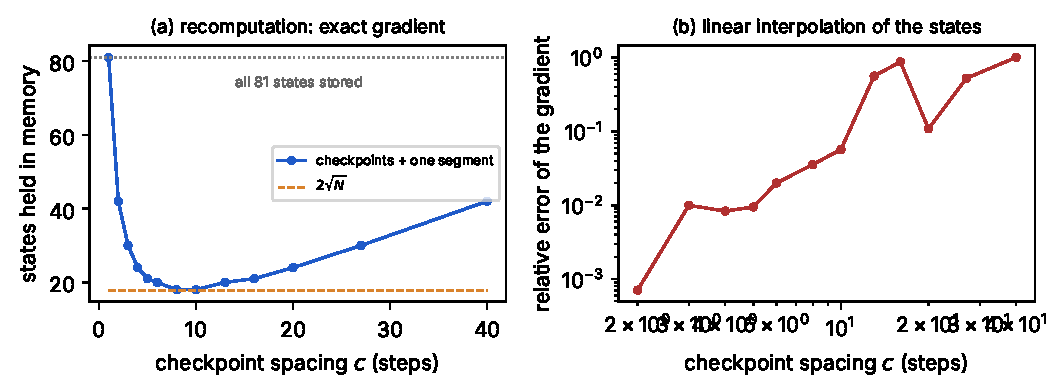
\includegraphics[width=0.85\textwidth]{figures/ch7/storage.pdf}
\caption{Truss, adjoint with checkpoints every $c$ steps. (a) States held in
memory with recomputation of the segments: the minimum is near
$c\approx\sqrt N$. (b) Relative error of the gradient when the states between
checkpoints are interpolated linearly in time: large and irregular, because the
interpolated states fall on the wrong side of the yield condition.}
\label{fig:id-storage}
\end{figure}

\subsection{Viscoplasticity, contact and the continuous adjoint}\label{ssec:id-vp-adj}
\index{adjoint state!viscoplasticity}\index{indentation!viscoplastic}%
Constantinescu and Tardieu~\cite{ConstantinescuTardieu2001b} derived the adjoint
of the indentation of a generalized standard material without hardening, with a
twice differentiable dual potential $\varphi^\ast(\sig;\vp)$ and frictionless
contact, from the Lagrangian of the time-discretized problem, with one adjoint
field per direct field, $(\vu^\star,\sig^\star,p^\star)$. Their result combines the
two previous sections.
\begin{itemize}
  \item \emph{The adjoint law is viscoelastic in reversed time.} In the reversed
  time $\tau=T-t$,
  \[
    \eps[\Delta\vu^\star]=\bbS:\Delta\sig^\star+\Delta t\,\mathbb{R}:\sig^\star,
    \qquad \mathbb{R}=\frac{\partial^2\varphi^\ast}{\partial\sig^2}\bigl(\sig(T-\tau)\bigr),
  \]
  a linear viscoelastic law of Maxwell type, anisotropic and heterogeneous, with
  coefficients taken from the direct solution. Since $\varphi^\ast$ is convex,
  $\mathbb R$ is symmetric positive semi-definite: the adjoint material is again
  a standard material. For a Maxwell material, $\varphi^\ast=\tfrac12\sig:\mathbb M:\sig$,
  it is the material itself.
  \item \emph{The terminal condition is an elastic problem} at $t=T$, and the
  adjoint is integrated from $T$ back to $0$.
  \item \emph{The adjoint is not a contact problem:} at each step it carries the
  Dirichlet datum $F^{\mathrm{calc}}_n-F^{\mathrm{exp}}_n$ on the contact zone of
  the direct step $n$, as in Section~\ref{sec:id-contact}.
  \item \emph{The gradient} is
  \[
    \nabla\mathcal J=\sum_n\int_\Omega\Bigl(\Delta\sig_n:\frac{\partial\bbS}{\partial\vp}:\sig^\star_n
    +\Delta t\,\frac{\partial^2\varphi^\ast}{\partial\sig\,\partial\vp}:\sig^\star_n\Bigr)\dd x
  \]
  (with the signs of~\cite{ConstantinescuTardieu2001b}).
  \item \emph{It needs $\varphi^\ast$ twice differentiable}: $m>1$ for Norton--Hoff.
  A gradient cost about $1.5$ direct computations, because the adjoint is linear
  and has no contact; the price is the storage of the direct fields.
\end{itemize}
For the Maxwell material, the identification of $E$ and the viscosity from
exact data converged to $0.02\%$ from starts five times too small or three times
too large; with $10\%$ noise, to $2.5\%$. For the Norton--Hoff material, $E$ was
identified to $1\%$ and $K$ to $1$--$10\%$, while $m$ and $\sY$ moved along a long
valley in which every identified curve fitted the data: the valley of
Figure~\ref{fig:id-norton}.

\paragraph{Differentiate, then discretize?}
\index{discrete adjoint}\index{continuous adjoint}%
The adjoint above was derived from a time-discrete Lagrangian, but with formal
manipulations (a first-order discrete integration by parts) and implemented with
its own time scheme; it agreed with finite differences to about $10\%$. In
poroelasticity, an adjoint derived in continuous time and then discretized
agreed with the direct differentiation to $1$--$3\%$~\cite{LecampionConstantinescu2005}.
The discrete adjoint of Box~7.4, obtained by differentiating the computation
itself, agrees to round-off (Table~\ref{tab:id-fd}). The lesson of Michaleris et
al.~\cite{MichalerisTortorelliVidal1994} is to \emph{discretize, then
differentiate}: the optimizer needs the gradient of the computed cost, not an
approximation of the gradient of the exact one.

\subsection{The rate-independent limit}\label{ssec:id-limit}
\index{kinks!plasticity}\index{biactive constraint!plasticity}%
As $m\to\infty$, or as the viscosity tends to zero, $\mathbb R$ concentrates on
the yield surface and the viscoplastic adjoint degenerates. The discrete
rate-independent computation has the structure of contact: at each step and
Gauss point the active set is plastic or elastic, the derivatives of
Section~\ref{prop:id-rm} are those of the active branch, and the cost is piecewise
smooth, with kinks where a point of the history is biactive. Lee and
Arora~\cite{LeeArora1995} discuss these discontinuities of the sensitivities in
elastoplastic structures. The mathematical theory is recent. For static
plasticity with linear kinematic hardening the solution map is directionally,
not Fr\'echet, differentiable, and the optimality conditions take the forms
called C-, B- and strong stationarity~\cite{HerzogMeyerWachsmuth2012,HerzogMeyerWachsmuth2013};
for the quasi-static evolution, Wachsmuth proved existence of optimal controls
and obtained optimality conditions through a viscous
regularization~\cite{Wachsmuth2012,Wachsmuth2015,Wachsmuth2016}. In practice:
\begin{itemize}
  \item the gradient of Boxes~7.3--7.4 is exact wherever no point is biactive,
  which is the generic case, and it is a one-sided derivative otherwise;
  \item a kink affects the convergence of a quasi-Newton method only near it, and
  Levenberg--Marquardt is robust to it;
  \item if the kinks matter, a viscous regularization (Section~\ref{sec:pn-vp})
  makes the cost smooth, at the price of a model error that vanishes with the
  viscosity.
\end{itemize}

\begin{figure}[h]
\centering
\begin{tikzpicture}[x=1.0cm,y=1cm,>=Latex]
  \foreach \x/\l in {0/t_0,2/t_1,4/t_{n-1},6/t_n,8/t_{N-1},10/t_N}
     {\node[below,font=\small] at (\x,-2.45) {$\l$};
      \draw[gray!40] (\x,0.85) -- (\x,-2.35);}
  \node[font=\sffamily\small,anchor=east] at (-0.2,0.6) {direct};
  \node[font=\sffamily\small,anchor=east] at (-0.2,-0.7) {sensitivities};
  \node[font=\sffamily\small,anchor=east] at (-0.2,-2.0) {adjoint};
  \foreach \a/\b in {0/2,4/6,8/10}
     {\draw[->,very thick,cu] (\a+0.1,0.6) -- (\b-0.1,0.6);
      \draw[->,thick,cphi] (\a+0.1,-0.55) -- (\b-0.1,-0.55);
      \draw[->,thick,cphi] (\a+0.1,-0.85) -- (\b-0.1,-0.85);
      \draw[<-,very thick,orange!80!black] (\a+0.1,-2.0) -- (\b-0.1,-2.0);}
  \foreach \a in {3,7} {\node[font=\small] at (\a,0.6) {$\cdots$};
     \node[font=\small] at (\a,-0.7) {$\cdots$}; \node[font=\small] at (\a,-2.0) {$\cdots$};}
  \foreach \x in {2,6,10} {\draw[->,thin,red!70!black,dashed] (\x,0.45) -- (\x,-1.85);}
  \node[font=\scriptsize,red!70!black,anchor=west] at (2.15,-1.35) {loads $\partial j_n/\partial\mat{u}_n$};
  \node[font=\scriptsize,cu,anchor=west] at (10.3,0.6) {stores $\mat{u}_n$, $\vz_n$, $\bbCalg_n$};
  \node[font=\scriptsize,cphi,anchor=west,align=left] at (10.3,-0.7) {$n_p$ right-hand sides,\\ same $\mat{K}^{\mathrm{alg}}_n$};
  \node[font=\scriptsize,orange!80!black,anchor=west,align=left] at (10.3,-2.0) {starts from $\boldsymbol\mu_N=\vzero$;\\ $(\mat{K}^{\mathrm{alg}}_n)\T\boldsymbol\lambda_n$, $\boldsymbol\mu_{n-1}$ from $\boldsymbol\mu_n$};
\end{tikzpicture}
\caption{Three sweeps through the same steps. The direct computation (blue)
marches forward and stores the state and the tangents. The direct differentiation
(green) marches forward with it, with $n_p$ right-hand sides per step. The adjoint
(orange) starts from $\boldsymbol\mu_N=\vzero$ after the last step and runs backward,
loaded at each step by the misfit of the observations of that step (red).}
\label{fig:id-sweeps}
\end{figure}

%======================================================================
\section{How the pieces fit together today}\label{sec:id-tools}
\index{automatic differentiation}\index{identification!software}%
\subsection{Five pieces}
An identification code is made of five pieces (Figure~\ref{fig:id-pipeline}),
whatever the software.

\paragraph{Experiment.} The measured observations $\mat{y}^m$, with their noise
levels $s_i$ and the loading $\ell$ that produced them (Section~\ref{ssec:id-def}).

\paragraph{Cost functional.} The distance between the computed and the measured
observations, here the output least squares~\eqref{eq:id-ols}, possibly
regularized. It is the only place where the data enter the computation.

\paragraph{Direct solver.} The computation of $\mat{y}(\vp;\ell)$: a finite element
code with the plasticity of Chapters~\ref{ch:pl}--\ref{ch:pl-num}, that is, the
nodal equilibrium solved by Newton's method with the return map at the Gauss
points.

\paragraph{Derivative layer.} The sensitivity matrix $\mat{S}$ or the gradient
$\nabla\mathcal J$, by direct differentiation (Box~7.3) or adjoint differentiation
(Box~7.4), written by hand or generated by automatic differentiation; finite
differences are the fallback. It uses the converged states and tangents of the
direct solver.

\paragraph{Driver.} The descent decision: from $\mathcal J(\vp_k)$ and its derivative,
choose the next parameters $\vp_{k+1}$ and decide when to stop. It is an optimizer
(Section~\ref{sec:id-algo}, Appendix~\ref{app:opt}), or a calibration tool which
adds the statistics of the result.

In the work of the 1990s and 2000s quoted in this chapter, these pieces were
written by hand in the language of a finite element code, for instance the
Gibiane language of Cast3M, with the operator \texttt{PASAPAS} reused to store
and refactorize the tangents~\cite{LecampionConstantinescuNguyen2002,ConstantinescuTardieu2001b}.
Today each piece exists as a library, and the main ones are listed in
Table~\ref{tab:id-tools}. The rest of the section explains what each one does,
and which of them were used for the exercises of this chapter.

\begin{table}[h]
\centering\small
\renewcommand{\arraystretch}{1.2}
\begin{tabular}{@{}>{\raggedright}p{2.6cm}>{\raggedright}p{5.4cm}>{\raggedright\arraybackslash}p{6.0cm}@{}}
\toprule
\sffamily tool & \sffamily what it is & \sffamily its role in an identification\\
\midrule
JAX & Python library: NumPy-like arrays with automatic differentiation (forward and reverse) and compilation & differentiates a return map or a whole small solver; gradients without hand derivation\\
SciPy (\texttt{optimize}) & Python library of scientific computing & driver: Nelder--Mead, BFGS, Levenberg--Marquardt with a user gradient or Jacobian\\
OpenTURNS & platform for uncertainty quantification (EDF, Airbus, Phimeca, IMACS, ONERA) & driver with statistics: calibration by least squares or Bayesian methods, posterior of $\vp$, sensitivity indices\\
FEniCSx (DOLFINx, UFL) & finite element library with symbolic weak forms & direct solver; symbolic tangents of the global problem\\
dolfinx-external-operator, dolfinx\_materials & extensions of FEniCSx for constitutive laws at the Gauss points & return map written in Python/JAX or MFront, tangent by automatic differentiation\\
pyadjoint (dolfin-adjoint, dolfinx-adjoint) & taping adjoint for FEniCS and Firedrake programs & derivative layer: reverse mode of a whole simulation, Taylor test\\
JAX-FEM & differentiable finite element solver written in JAX & direct solver and derivative layer in one program\\
MFront, MTest & code generator for constitutive laws; test of a law on a material point & local level: one return map for several codes; MTest is a direct solver for homogeneous tests\\
code\_aster, Cast3M & general finite element codes (EDF, CEA) & direct solver; \texttt{MACR\_RECAL} of code\_aster: Levenberg--Marquardt with finite differences\\
\bottomrule
\end{tabular}
\caption{Software for the pieces of an identification code; websites and
starting examples are listed in Section~\ref{ssec:id-links}.}
\label{tab:id-tools}
\end{table}

\subsection{Automatic differentiation}
\index{automatic differentiation!forward and reverse mode}%
\paragraph{Two modes, two methods of this chapter.}
A program is a composition of elementary operations, and the chain rule can be
applied to it mechanically. \emph{Forward mode} propagates derivatives with the
computation, one input direction at a time: it is the direct differentiation of
Box~7.3. \emph{Reverse mode} records the computation on a \emph{tape} and
propagates the derivative of one output backward: it is the adjoint of Box~7.4,
with the tape in the role of the stored history~\cite{GriewankWalther2008}. The
two are not new methods; they are the methods of this chapter, generated by the
computer.

\paragraph{Differentiate the solution, not the iterations.}
Automatic differentiation differentiates the \emph{algorithm} that was run,
including the iterations of Newton's method. If the iterations were stopped
early, the result is the derivative of an unconverged iterate, not of the
solution. The truss shows it. Written with JAX and differentiated in reverse mode,
the cost of Section~\ref{sec:id-algo} with a fixed number of Newton iterations per
step gives a gradient that differs from the adjoint of Box~7.4 by $2\%$ with one
iteration, and by $10^{-16}$ with two, the number this piecewise-linear problem
needs to converge (Exercise~\ref{exo:id-tools}). Large codes therefore do not
differentiate through the iterations: they use the \emph{implicit} derivative at
the converged solution, which is again Boxes~7.3--7.4, and use automatic
differentiation for the local pieces, the return map and its derivatives.

\paragraph{The local level.}
Differentiating a return map by hand is error-prone; the derivatives
$\bbCalg$, $\hat\sig_{,\vz}$, $\hat\sig_{,\vp}$ of Section~\ref{sec:id-path} are
exactly what automatic or symbolic differentiation delivers. Rothe and
Hartmann~\cite{RotheHartmann2015} compare analytical, numerical and automatic
derivatives for stresses and consistent tangents; Korelc and
Wriggers~\cite{KorelcWriggers2016} generate element and material routines with
their sensitivities symbolically (AceGen). The code generator
MFront~\cite{HelferEtAl2015} writes the return map and its tangent once for
several finite element codes.

\subsection{Direct solvers and derivative layers}
\index{FEniCS}\index{dolfin-adjoint}%
\paragraph{FEniCSx.}
In FEniCSx (DOLFINx), the weak form is written in the language UFL, which
differentiates forms symbolically: the tangent of the global Newton method is
the derivative of the residual form~\cite{AlnaesEtAl2014}. A constitutive law
evaluated at the Gauss points enters as an \emph{external operator}, a Python
function whose derivative may be obtained by automatic differentiation with
JAX~\cite{LatyshevEtAl2025}; elastoplastic return maps and their consistent
tangents are written this way, or called from MFront through dolfinx\_materials.

\paragraph{pyadjoint.}
The adjoint of a whole FEniCS or Firedrake computation is provided by pyadjoint
(dolfin-adjoint), which tapes the solves of the program and solves the adjoint
equations backward~\cite{FarrellEtAl2013,MituschFunkeDokken2019}: a
\texttt{ReducedFunctional} returns $\mathcal J$ and $\nabla\mathcal J$, and a
\texttt{taylor\_test} checks the gradient (Box~7.5). Its port to DOLFINx,
dolfinx-adjoint, is recent.
\draftnote{The DOLFINx pipeline (external operator for the return map +
dolfinx-adjoint for the backward sweep) is described from the documentation and
has not been tested here; in particular, whether the adjoint layer handles the
history variables stored at the Gauss points must be checked on the truss or on
the cylinder of Chapter~\ref{ch:pl-num} before this paragraph is final.}

\paragraph{Differentiable solvers.}
Solvers written entirely in JAX, such as JAX-FEM~\cite{XueEtAl2023}, apply
reverse mode with implicit differentiation at the Newton solution to the whole
simulation; a $J_2$ plasticity example is part of its documentation.

\subsection{Drivers}
\index{OpenTURNS}\index{optimization libraries}%
\paragraph{Optimizers.}
The driver needs the values, and the gradient or the sensitivities. General
optimizers such as those of SciPy~\cite{VirtanenEtAl2020} (Nelder--Mead, BFGS,
Levenberg--Marquardt) accept a gradient or a Jacobian supplied by the user; the
algorithms are explained in Appendix~\ref{app:opt}. Finite element codes ship
identification tools of the same kind: the macro command \texttt{MACR\_RECAL} of
code\_aster runs Levenberg--Marquardt with finite-difference sensitivities.

\paragraph{Calibration with statistics.}
The uncertainty platform OpenTURNS~\cite{BaudinEtAl2017} adds the statistical
layer. A model wrapped as a Python function, with its gradient if available, is
calibrated by nonlinear least squares, by a Gaussian (Bayesian) linearization, or
by Markov chain Monte Carlo, and the result comes with a posterior distribution of
the parameters, the statistical form of Section~\ref{prop:id-GN}. Its sensitivity
tools (Sobol indices) answer the question of Section~\ref{ssec:id-tell} globally,
over a range of parameters rather than at one point.

\paragraph{The truss with OpenTURNS.}
On the truss, the observation map of Section~\ref{sec:id-algo}, wrapped with the
direct differentiation of Box~7.3 as its gradient and calibrated by OpenTURNS with
Levenberg--Marquardt, returns the same parameters as in Section~\ref{sec:id-algo}
in 14 direct computations, with the posterior standard deviations
$(0.6\%,\,0.09\%,\,0.8\%)$ of $(\log E,\log\sY,\log H)$ (Exercise~\ref{exo:id-tools}).
The correlation of $\sY$ and $H$ of Section~\ref{ssec:id-sens} is visible again:
$\sY$ alone is determined to $0.1\%$, but the combination along the weak
direction only to $1\%$. One setting matters: the default optimizer of the
calibration stopped early on this problem, and Levenberg--Marquardt had to be
selected explicitly.

\subsection{Websites and where to start}\label{ssec:id-links}
\index{identification!software (websites)}%
The scripts of Exercises~\ref{exo:id-truss}--\ref{exo:id-tools} use NumPy and
SciPy, JAX~0.11 and OpenTURNS~1.27. The following pages are good entry points
(checked in October 2026).
\begin{itemize}
  \item \textbf{JAX}: \url{https://docs.jax.dev}. Start with the page
  ``Automatic differentiation''; ``Custom derivative rules'' shows how to give a
  function its own derivative, for instance an implicit one at a converged
  solution. Our script: Exercise~\ref{exo:id-tools}.
  \item \textbf{SciPy}: \url{https://docs.scipy.org/doc/scipy/tutorial/optimize.html},
  section ``Least-squares minimization'' (\texttt{least\_squares} with a
  user-supplied Jacobian). Our scripts: Exercises~\ref{exo:id-truss}--\ref{exo:id-norton}.
  \item \textbf{OpenTURNS}: \url{https://openturns.github.io/www/}. In the
  documentation, the gallery ``Calibration'' contains ``Calibration of the
  Chaboche mechanical model'', a uniaxial elastoplastic law calibrated by least
  squares and by Bayesian methods: the closest published example to this
  chapter. Our script: Exercise~\ref{exo:id-tools}.
  \item \textbf{FEniCSx}: \url{https://fenicsproject.org}; the tutorial of
  J.~S.~Dokken, \url{https://jsdokken.com/dolfinx-tutorial/}; the numerical tours of
  J.~Bleyer, \url{https://bleyerj.github.io/comet-fenicsx/}, with the tour
  ``Elasto-plastic analysis of a 2D von Mises material''.
  \item \textbf{dolfinx-external-operator}:
  \url{https://a-latyshev.github.io/dolfinx-external-operator/}, demos of von Mises
  and Mohr--Coulomb plasticity; \textbf{dolfinx\_materials}:
  \url{https://bleyerj.github.io/dolfinx_materials/}.
  \item \textbf{pyadjoint}: \url{https://pyadjoint.org}, and the tutorial ``First
  steps'' of dolfin-adjoint; \textbf{dolfinx-adjoint}:
  \url{https://github.com/scientificcomputing/dolfinx-adjoint}.
  \item \textbf{JAX-FEM}: \url{https://deepmodeling.github.io/jax-fem/}, example
  ``Plasticity''.
  \item \textbf{MFront}: \url{https://thelfer.github.io/tfel/web/index.html}; MTest,
  \url{https://thelfer.github.io/tfel/web/mtest.html}, can be wrapped in a driver
  to fit parameters on homogeneous tests.
  \item \textbf{code\_aster}: \url{https://code-aster.org} (command
  \texttt{MACR\_RECAL}, document U4.73.02); \textbf{Cast3M}:
  \url{https://www-cast3m.cea.fr}.
\end{itemize}
None of these examples identifies an elastoplastic law with an adjoint through a
finite element history; the chapter's truss scripts do it on the smallest
structure, and the same structure scales to finite elements by replacing the
fibres by Gauss points and the $2\times2$ tangent by the assembled one.

\begin{figure}[h]
\centering
\begin{tikzpicture}[>=Latex]
  \node[smallbox,stat,minimum width=3.4cm,minimum height=1.3cm] (exp) at (0,0) {\textbf{experiment}\\ \footnotesize measured $\mat{y}^m$};
  \node[smallbox,minimum width=3.4cm,minimum height=1.3cm] (cost) at (5.6,0) {\textbf{cost functional}\\ \footnotesize $\mathcal J(\vp)$};
  \node[smallbox,kin,minimum width=3.4cm,minimum height=1.3cm] (fem) at (11.2,0) {\textbf{direct solver}\\ \footnotesize finite elements + plasticity};
  \node[smallbox,key,minimum width=3.4cm,minimum height=1.3cm] (drv) at (5.6,-3.4) {\textbf{driver}\\ \footnotesize descent decision};
  \node[smallbox,minimum width=3.4cm,minimum height=1.3cm] (der) at (11.2,-3.4) {\textbf{derivative layer}\\ \footnotesize direct or adjoint\\ \footnotesize differentiation};
  \draw[arr] (exp) -- (cost) node[midway,above,font=\small] {$\mat{y}^m$};
  \draw[arr] (fem) -- (cost) node[midway,above,font=\small] {$\mat{y}(\vp_k)$};
  \draw[arr] (cost) -- (drv) node[midway,left,font=\small] {$\mathcal J(\vp_k)$};
  \draw[arr] (fem) -- (der) node[midway,right,font=\small,align=left] {states,\\ tangents};
  \draw[arr] (der) -- (drv) node[midway,below,font=\small] {$\mat{S}$ or $\nabla\mathcal J$};
  \draw[arr] (drv.north east) -- (fem.south west) node[pos=0.55,above left,font=\small] {$\vp_{k+1}$};
\end{tikzpicture}
\caption{The five pieces of an identification code. The driver takes the descent
decision from the cost and its derivative; the direct solver and the derivative
layer compute them for the parameters it proposes.}
\label{fig:id-pipeline}
\end{figure}

\begin{gbox}{Box 7.5\quad Checking a gradient: the Taylor test}
\index{Taylor test}%
\begin{enumerate}[label=\textbf{\arabic*.},leftmargin=1.6em]
  \item \textbf{Direction.} Choose $\vp$ and a random direction $\delta\vp$.
  \item \textbf{Remainders.} For $h=10^{-1},10^{-2},\dots$, compute
  $e_0(h)=|\mathcal J(\vp+h\delta\vp)-\mathcal J(\vp)|$ and
  $e_1(h)=|\mathcal J(\vp+h\delta\vp)-\mathcal J(\vp)-h\nabla\mathcal J\cdot\delta\vp|$.
  \item \textbf{Rates.} $e_0$ must decrease like $h$ and $e_1$ like $h^2$, until
  round-off. A rate $1$ for $e_1$ means a wrong gradient; a rate between $1$ and
  $2$ often means a kink (a biactive point) or an unconverged direct solve.
\end{enumerate}
\end{gbox}

%======================================================================
\framepart{Summary}
\begin{gbox*}
\begin{itemize}
  \item \textbf{Setting}: model with parameters $\vp$, experiment (imposed
  data), observations (other data), observation map $\vp\mapsto\mat{y}(\vp)$.
  Inactive mechanisms are invisible; invariances give lumped parameters; each
  part of the history informs some parameters.
  \item \textbf{Minimization}: output least squares
  $\mathcal J=\tfrac12\norm{\mat{r}}^2$ with scaled residuals; the sensitivity matrix
  $\mat{S}=\partial\mat{r}/\partial\vp$; the eigenvalues of $\mat{S}\T\mat{S}$ give
  identifiability and the uncertainty $1/\sqrt{\lambda_k}$ along each direction.
  \item \textbf{Algorithms}: Nelder--Mead needs only values and fails on curved
  valleys; Levenberg--Marquardt needs $\mat{S}$ (direct differentiation); BFGS
  needs $\nabla\mathcal J$ (adjoint). Start where the mechanisms are active.
  \item \textbf{Gradients}: finite differences (cost $n_p$, accuracy
  $\sqrt\epsilon$); direct differentiation (forward, $n_p$ right-hand sides with the
  factorized tangent); adjoint (one backward solve with the transposed
  operator, any number of parameters).
  \item \textbf{Contact}: under strict complementarity the adjoint is a linear
  problem with Dirichlet data on the contact zone of the direct solution; biactive
  nodes give kinks, of the order of the mesh size here.
  \item \textbf{Plasticity}: the derivative of the return map is that of the
  active branch; the adjoint runs backward with the transposed consistent
  tangents and a local memory $\boldsymbol\mu$; viscoplastic adjoints are viscoelastic
  in reversed time. Discretize, then differentiate.
  \item \textbf{Tools}: forward and reverse automatic differentiation are the direct
  and adjoint methods; differentiate the converged solution, not the iterations;
  FE code, derivative layer and driver are separate layers; check every gradient
  with a Taylor test.
\end{itemize}
\end{gbox*}

\framepart{Exercises}\label{sec:id-exo}
Short questions come first, then problems on the three model problems. The
computational problems use the module \texttt{id\_core}, presented on
page~\pageref{sec:id-aux}; the results are stated in words first, and the
scripts are printed after them.

\framesub{Short questions}

\exercise{What a tension test can tell}\label{exo:id-q-tension}
\index{identifiability!exercise}%
A filament with combined linear hardening ($K$ isotropic, $H$ kinematic,
Section~\ref{ssec:pl-1d-kin}) is pulled monotonically. (a) Show that the
stress--strain curve depends on $E$, $\sY$ and $K+H$ only. (b) After a strain
$\varepsilon_1$ in tension, the filament is unloaded and compressed. At which stress
does it yield again? Show that this reverse yield stress separates $K$ and $H$.
\begin{solution}
(a) On the plastic branch $\dg=f^\trial/(E+K+H)$ (Box~5.1) and the slope is
$E(K+H)/(E+K+H)$: only the sum enters. (b) At the end of the tensile branch,
$\sigma_1=\sY+(K+H)\alpha_1$ and $q_1=H\alpha_1$, where $\alpha_1$ is the accumulated
plastic strain. Reverse yield occurs at $\sigma-q_1=-(\sY+K\alpha_1)$, i.e.\
$\sigma=H\alpha_1-\sY-K\alpha_1$. Knowing $\sY$ and $K+H$ from the tensile branch,
this value gives $H-K$, hence both. Purely kinematic hardening yields again at
$\sigma_1-2\sY$, purely isotropic at $-\sigma_1$: the Bauschinger effect is the
information.
\end{solution}

\exercise{Two springs}\label{exo:id-q-springs}
\index{springs!identification (exercise)}%
In the two-spring example of Section~\ref{sec:id-grad}, (a) compute
$\partial\mat{u}/\partial k_2$ by direct differentiation; (b) check the adjoint
gradient; (c) add a second experiment, a force $f$ at the middle node, with the
measured displacement $u_1'$, and write the Gauss--Newton matrix of the two
experiments. When is it invertible?
\begin{solution}
(a) $\partial\mat{K}/\partial k_2=\begin{bmatrix}1&-1\\-1&1\end{bmatrix}$, the
pseudo-load is $-\partial_{k_2}\mat{K}\,\mat{u}=-(u_1-u_2)(1,-1)=(f/k_2)(1,-1)$, and
$\mat{K}\,\partial\mat{u}/\partial k_2=(f/k_2,-f/k_2)$ gives
$\partial\mat{u}/\partial k_2=(0,-f/k_2^2)$: the first spring does not feel the
second. (b) As in the text. (c) The second experiment gives $u_1'=f/k_1$, with
$\partial u_1'/\partial(k_1,k_2)=(-f/k_1^2,0)$. With unit scales,
$\mat{S}=-f\begin{bmatrix}1/k_1^2&1/k_2^2\\1/k_1^2&0\end{bmatrix}$, whose determinant
$-f^2/(k_1^2k_2^2)$ never vanishes: $\mat{S}\T\mat{S}$ is invertible, the two
experiments together identify both springs.
\end{solution}

\exercise{The step of a finite difference}\label{exo:id-q-fd}
\index{finite differences!exercise}%
The cost is computed with the relative accuracy $\epsilon$. (a) Show that the error
of the forward difference is at most
$\tfrac12h|\mathcal J''|+2\epsilon|\mathcal J|/h$, and find the best step. (b) What is the
best step for the central difference? (c) Read Table~\ref{tab:id-fd} with these
estimates.
\begin{solution}
(a) Taylor: $(\mathcal J(p+h)-\mathcal J(p))/h=\mathcal J'+\tfrac12h\mathcal J''(\xi)$; each value carries
an error $\epsilon|\mathcal J|$, divided by $h$. The sum is smallest for
$h=2\sqrt{\epsilon|\mathcal J|/|\mathcal J''|}$, of the order of $\sqrt\epsilon$ in relative terms,
and the error is then of order $\sqrt\epsilon$. (b) The truncation error is
$\tfrac16h^2|\mathcal J'''|$: $h\sim\epsilon^{1/3}$, error $\epsilon^{2/3}$. (c) With
$\epsilon\approx10^{-15}$, the forward difference is best near $h=10^{-8}$ (seven digits),
the central one gives eight digits at $10^{-6}$; the error grows on both sides, by
truncation for $h=10^{-2}$ and by round-off for $h=10^{-10}$. With an iterative
solver stopped at $10^{-6}$, $\epsilon=10^{-6}$ and no step gives more than three
digits.
\end{solution}

\exercise{A kink in one step}\label{exo:id-q-kink}
\index{kinks!exercise}%
One step of the filament with linear kinematic hardening starts from the virgin
state and reaches the strain $\varepsilon$. (a) Write $\sigma$ as a function of $\sY$.
(b) Compute $\partial\sigma/\partial\sY$ on both sides of $\sY=E\varepsilon$. (c) Which
value do Boxes~7.3--7.4 return at $\sY=E\varepsilon$? Why does it rarely matter?
\begin{solution}
(a) $\sigma=E\varepsilon$ if $E\varepsilon\le\sY$; otherwise
$\varepsilon^p=(E\varepsilon-\sY)/(E+H)$ and $\sigma=E(\varepsilon-\varepsilon^p)=(EH\varepsilon+E\sY)/(E+H)$.
(b) $0$ for $\sY>E\varepsilon$ (elastic), $E/(E+H)$ for $\sY<E\varepsilon$ (plastic): a
kink. (c) The derivative of the branch chosen by the test $f^\trial>0$ of the code:
the elastic one if $f^\trial=0$ is classified elastic. The kink is met only if a
point of the history is exactly at yield without flowing; the set of such
parameters has measure zero, and a minimization passes it like a corner of a
piecewise-smooth function.
\end{solution}

\exercise{Homogeneity of the indentation force}\label{exo:id-q-homog}
\index{indentation!homogeneity}%
(a) Show that the force of the membrane satisfies $F(\lambda k_f,\lambda T_m;U)=\lambda F(k_f,T_m;U)$.
(b) Deduce that $\partial\log F/\partial\log k_f+\partial\log F/\partial\log T_m=1$.
(c) Why can one depth not identify both parameters? Which elastic constants of a
homogeneous isotropic half-space indented by a rigid punch can a force--depth
curve determine?
\begin{solution}
(a) The constraint $\mat{u}\ge\mat{d}$ does not depend on the parameters, and
$\mat{K}$ is multiplied by $\lambda$: the minimizer of~\eqref{eq:id-contact} is unchanged
and the forces $\mat{t}=\mat{K}\mat{u}$ are multiplied by $\lambda$. (b) Differentiate
with respect to $\lambda$ at $\lambda=1$ (Euler's identity). (c) One depth gives one
number, which fixes one combination; the other combination is the length
$\sqrt{T_m/k_f}$, which shapes the dependence on the depth. For the half-space, the
same argument shows that the curve depends on the moduli through the contact
modulus $E/(1-\nu^2)$ only: $E$ and $\nu$ cannot be separated by a frictionless
indentation of a homogeneous elastic body.
\end{solution}

\exercise{Which tangent?}\label{exo:id-q-tangent}
\index{consistent tangent!sensitivity (exercise)}%
A filament with linear kinematic hardening is pulled in one plastic step from the
virgin state to the strain $\varepsilon$. (a) Compute $\partial\sigma/\partial\sY$ exactly. (b)
A structure made of such filaments is computed with the elastic stiffness in the
global iterations (Box~6.1). Which matrix must the sensitivity problem use? (c)
What is wrong with the continuum tangent for a step that starts elastic and ends
plastic?
\begin{solution}
(a) $\varepsilon^p=(E\varepsilon-\sY)/(E+H)$, $\sigma=E(\varepsilon-\varepsilon^p)$, so
$\partial\sigma/\partial\sY=E/(E+H)$ at fixed $\varepsilon$; in a structure the
strain changes too, through $\mat{K}^{\mathrm{alg}}\delta\mat{u}=-\sum\mat{B}\T\hat\sig_{,\sY}$.
(b) The consistent tangent at the converged state, with $E_t=EH/(E+H)$ in the
plastic fibres: the iterations that found the solution play no role in its
derivative. (c) The continuum tangent of the start of the step is elastic, $E$,
whereas the discrete update is plastic: the derivative of the computed stress is
$E_t$. The two coincide only in the limit of small steps.
\end{solution}

\exercise{What a gradient costs}\label{exo:id-q-cost}
\index{gradient!cost (exercise)}%
A model has $10^5$ unknowns, its direct computation 200 steps of 3 Newton
iterations, and $n_p=4$ parameters. Count the factorizations and the solves per
gradient for central differences, direct differentiation and adjoint. Which
method would you choose for $n_p=4$ with Levenberg--Marquardt? For a field of
$10^4$ moduli?
\begin{solution}
Direct: 600 factorizations and solves. Central differences: 8 more direct
computations, 4800 factorizations. Direct differentiation: no new factorization,
$4\times200$ solves with stored factors. Adjoint: no new factorization if the factors
are stored (or 200 refactorizations if only the states are stored), 200 solves,
and the storage of the history. For $n_p=4$ with Levenberg--Marquardt, direct
differentiation: it gives $\mat{S}$ for the price of 800 back-substitutions. For
$10^4$ moduli, the adjoint: one backward sweep instead of $10^4$ right-hand sides
per step.
\end{solution}

\exercise{The memory of the adjoint}\label{exo:id-q-memory}
\index{adjoint state!memory (exercise)}%
For the filament with linear kinematic hardening, use Box~7.4 to show that
$\mu_{n-1}=0$ after a plastic step and $\mu_{n-1}=\mu_n+E\,(\mat{B}\boldsymbol\lambda_n)$
after an elastic step. Interpret both cases in terms of the dependence of the
direct solution on its history.
\begin{solution}
Plastic step: $\hat z_{,z}=0$ and $\hat\sigma_{,z}=0$ (Section~\ref{sec:id-path}), so step~5
gives $\mu_{n-1}=0$. Elastic step: $\hat z_{,z}=1$ and $\hat\sigma_{,z}=-E$, so
$\mu_{n-1}=\mu_n+E\,\mat{B}\boldsymbol\lambda_n$. The adjoint multiplier is the sensitivity of
the cost to the plastic strain left at $t_{n-1}$. A plastic step recomputes the
plastic strain from the current strain alone and forgets the past: nothing done
before can influence the later observations through it. An elastic step keeps the
plastic strain and turns it into stress: the influence passes through it, plus
the direct effect of the stress at that step.
\end{solution}

\framesub{The module \texttt{id\_core}}
\phantomsection\label{sec:id-aux}%
\index{identification!Python implementation}%
The computational problems import one module, \texttt{id\_core}. Its function
\texttt{filament\_kin} is the return map of the filament with linear kinematic
hardening together with all its derivatives with respect to the strain, the
history and the parameters $(E,\sY,H)$. The class \texttt{Truss} computes the truss
of Chapter~\ref{ch:pl-cyc} step by step with Newton's method, and its cost and
gradient by finite differences, by direct differentiation (Box~7.3) and by the
adjoint (Box~7.4). The function \texttt{norton\_relax} integrates the Norton--Hoff
filament with its sensitivities, \texttt{Membrane} solves the indentation of the
membrane by a primal--dual active-set method and computes the derivative of the
force by the adjoint of Section~\ref{sec:id-contact}, and \texttt{gauss\_newton}
returns the eigenvalues and the correlations of Section~\ref{ssec:id-sens}.
\lstinputlisting[firstline=4]{python/examples/ch7/id_core.py}

\framesub{Problems}

\exercise{Identification of the truss}\label{exo:id-truss}
\index{three-bar truss!identification (exercise)}%
For the truss of Section~\ref{ssec:id-models} with noisy measurements: (a) compute
the gradient of the cost at $\vp=(0.9,1.2,1.5)\,\vp_{\mathrm{true}}$ by forward
differences with relative steps $10^{-2},\dots,10^{-10}$, by central differences,
by direct differentiation and by the adjoint; (b) compute the Gauss--Newton matrix
at the true parameters, for this loading and for the elastic loading
$Q_1=N_0\sin t$; (c) identify $(E,\sY,H)$ with Nelder--Mead, BFGS with the adjoint
gradient and Levenberg--Marquardt with the direct differentiation, from
$\vp_0=(0.7,1.5,3.0)$ and $(0.7,1.2,3.0)\times\vp_{\mathrm{true}}$, and count the
computations.
\begin{solution}
(a) Table~\ref{tab:id-fd}: the two exact methods agree with each other to all
digits and with the central difference to eight. (b) Eigenvalues
$(53,\,137,\,1.0\times10^5)$ in $\log\vp$; weakest direction
$(0.41,-0.11,0.91)$; correlation of $\sY$ and $H$ $-0.974$. Under the elastic loading,
$(0,\,0,\,13.7)$. (c) From the first start the truss stays elastic: the derivatives
with respect to $\sY$ and $H$ vanish and all the methods stop with $E=0.44E_{\mathrm{true}}$
($\mathcal J=522$). From the second start, Levenberg--Marquardt converges in 14 direct
computations and 11 sensitivity computations, BFGS in 28 direct and 28 adjoint
computations, both to $(1.0022,\,0.9992,\,1.0036)\,\vp_{\mathrm{true}}$ with
$\mathcal J=0.291$; Nelder--Mead stops after 1210 direct computations at
$(0.43,\,1.19,\,0)$ with $\mathcal J=453$.
\lstinputlisting[firstline=4]{python/examples/ch7/exo_truss_id.py}
\end{solution}

\exercise{Indentation of a membrane}\label{exo:id-indent}
\index{indentation!exercise}%
(a) Check the adjoint derivative~\eqref{eq:id-contact-grad} of the force against
central differences at several depths and parameters. (b) Compute the relative
sensitivities $\partial\log F/\partial\log(k_f,T_m)$ at $U=0.02$ and $U=0.2$. (c) Identify
$(k_f,T_m)$ from the forces at these two depths, from four starts. (d) Measure the
jumps of $\partial F/\partial k_f$ for $k_f\in[2,6]$ at $U=0.1$ on four meshes.
\begin{solution}
(a) Table~\ref{tab:id-contact}. (b) $(0.448,0.552)$ and $(0.544,0.456)$; each row
adds up to one (Exercise~\ref{exo:id-q-homog}). (c) Levenberg--Marquardt returns the
true values from the four starts in 8 to 23 iterations. (d) No change of the contact
zone on the coarsest mesh ($h=0.05$) in this range; then one, three and six changes,
with the largest jumps $3.4\%$, $1.9\%$, $0.9\%$ for $h=0.025$, $0.0125$, $0.0063$.
\lstinputlisting[firstline=5]{python/examples/ch7/exo_indentation.py}
\end{solution}

\exercise{Relaxation of a Norton--Hoff filament}\label{exo:id-norton}
\index{Norton--Hoff law!exercise}%
(a) Derive the sensitivities of the backward Euler update of~\eqref{eq:id-norton}
with respect to $(E,\sY,K,m)$, by differentiating the scalar equation
$x-x^\trial+E\Delta t\,\mac{(x-\sY)/K}^m=0$ for $x=|\sigma_n|$. (b) For holds of 10,
100 and 1000\,s, compute the Gauss--Newton matrix and the weakest direction.
(c) Identify the four parameters from data with $1\%$ noise, from three starts.
\begin{solution}
(a) With $y=(x-\sY)/K$ and $g=\Delta t\,y^m$:
$(1+Eg_x)\,\delta x=\delta x^\trial-g\,\delta E-E(g_{\sY}\delta\sY+g_K\delta K+g_m\delta m)$,
where $g_x=-g_{\sY}=m\Delta t\,y^{m-1}/K$, $g_K=-y\,g_x$, $g_m=g\log y$, and
$\delta x^\trial=s\,[(\varepsilon_n-\varepsilon^{vp}_{n-1})\delta E-E\,\delta\varepsilon^{vp}_{n-1}]$;
then $\delta\varepsilon^{vp}_n=\delta\varepsilon^{vp}_{n-1}+s(g_x\delta x+\delta_{\vp}g)$.
For $m>1$ the update is differentiable also at the threshold. (b)
Table~\ref{tab:id-norton}. (c) The three starts converge to the same point, with
an rms misfit at the noise level (2.6 to 2.9\,MPa): $(1.00,\,1.025,\,1.085,\,0.922)$
for the hold of 10\,s and $(0.999,\,0.984,\,0.927,\,1.071)$ for 1000\,s. The errors on
$K$ and $m$ lie along the weakest direction and are of the size predicted by its
eigenvalue.
\lstinputlisting[firstline=4]{python/examples/ch7/exo_norton.py}
\end{solution}

\exercise{What the adjoint must store}\label{exo:id-storage}
\index{checkpointing!exercise}%
For the truss at $\vp=(0.9,1.2,1.5)\,\vp_{\mathrm{true}}$, compute the adjoint gradient
(a) with all the states stored; (b) with a checkpoint every $c$ steps and the
segments recomputed by Newton; (c) with the states interpolated linearly between
the checkpoints. Compare memory, extra computation and error for
$c=1,2,4,\dots,40$. (d) Count the distinct patterns of plastic bars along the
history at $\vp$ and at $\vp_{\mathrm{true}}$.
\begin{solution}
(b) is exact for every $c$, at the price of one extra forward sweep (80 steps);
the number of states held is $N/c$ checkpoints plus one segment, smallest (18) for
$c=8$ to $10$. (c) costs nothing more but the error grows quickly and
irregularly: $7\times10^{-4}$ ($c=2$), $8\times10^{-3}$ ($c=4$), $4\times10^{-2}$ ($c=8$),
$1$ ($c=40$). (d) At $\vp$ only bar~3 yields: 16 plastic steps, 2 patterns, 4
changes; at $\vp_{\mathrm{true}}$, 38 plastic steps, 6 patterns, 12 changes. With
linear hardening, these few patterns give all the consistent tangents.
\lstinputlisting[firstline=4]{python/examples/ch7/exo_storage.py}
\end{solution}

\exercise{Automatic differentiation and a calibration driver}\label{exo:id-tools}
\index{automatic differentiation!exercise}\index{OpenTURNS!exercise}%
(a) Write the cost of the truss with JAX, with a fixed number of Newton iterations
per step, and compare its reverse-mode gradient with the adjoint of Box~7.4 for 1,
2 and 4 iterations. (b) Calibrate $(E,\sY,H)$ with OpenTURNS, wrapping the
observation map and its direct-differentiation gradient. Compare the posterior
standard deviations with the Gauss--Newton estimate of Section~\ref{ssec:id-sens}.
Algorithm~\ref{alg:id-adjoint} summarizes the adjoint that both computations
reproduce.
\begin{solution}
(a) The relative gap between the JAX gradient and the adjoint is $2\times10^{-2}$ with
one Newton iteration per step, $2\times10^{-16}$ with two and $2\times10^{-19}$ with four:
reverse mode differentiates the iterations that were run. (b) Levenberg--Marquardt
(CMinpack) converges in 14 direct computations to
$(1.0022,\,0.9992,\,1.0036)\,\vp_{\mathrm{true}}$; the posterior standard deviations of
$\log\vp$ are $(0.0059,\,0.0009,\,0.0079)$, consistent with the eigenvalues of
Exercise~\ref{exo:id-truss}. The scripts were run with JAX~0.11 and
OpenTURNS~1.27.
\begin{algorithm}[H]
\caption{Discrete adjoint of an incremental elastoplastic computation}\label{alg:id-adjoint}
\begin{algorithmic}[1]
\Require converged direct steps $n=1..N$: tangents $\mat{K}^{\mathrm{alg}}_n$, return-map derivatives at each Gauss point, observations $j_n$
\Ensure $\nabla\mathcal J$
\State $\boldsymbol\mu\gets\vzero$ at every Gauss point;\ \ $\mat{g}\gets\vzero$ \Comment{terminal condition}
\For{$n=N,N-1,\dots,1$}
  \State solve $(\mat{K}^{\mathrm{alg}}_n)\T\boldsymbol\lambda=\partial j_n/\partial\mat{u}_n+\sum_e\int\mat{B}\T\hat\vz_{,\eps}\T\boldsymbol\mu$
  \State $\mat{g}\gets\mat{g}-\int\hat\sig_{,\vp}\T\mat{B}\boldsymbol\lambda+\int\hat\vz_{,\vp}\T\boldsymbol\mu$
  \State $\boldsymbol\mu\gets\hat\vz_{,\vz}\T\boldsymbol\mu-\hat\sig_{,\vz}\T\mat{B}\boldsymbol\lambda$ at every Gauss point \Comment{memory, backward}
\EndFor
\State \Return $\mat{g}$
\end{algorithmic}
\end{algorithm}
\lstinputlisting[firstline=3]{python/examples/ch7/exo_jax_truss.py}
\lstinputlisting[firstline=4]{python/examples/ch7/exo_openturns_truss.py}
\end{solution}

\begin{chapterbib}{99}
\bibitem{AlnaesEtAl2014} M.~S.~Aln\ae s, A.~Logg, K.~B.~{\O}lgaard, M.~E.~Rognes, G.~N.~Wells, Unified Form Language: a domain-specific language for weak formulations of partial differential equations, \emph{ACM Trans. Math. Software} 40 (2014) art.~9.
\bibitem{AndradeCamposEtAl2007} A.~Andrade-Campos, S.~Thuillier, P.~Pilvin, F.~Teixeira-Dias, On the determination of material parameters for internal variable thermoelastic--viscoplastic constitutive models, \emph{Int. J. Plasticity} 23 (2007) 1349--1379.
\bibitem{BaudinEtAl2017} M.~Baudin, A.~Dutfoy, B.~Iooss, A.-L.~Popelin, OpenTURNS: an industrial software for uncertainty quantification in simulation, in R.~Ghanem et al.\ (eds.), \emph{Handbook of Uncertainty Quantification}, Springer, 2017, 2001--2038.
\bibitem{BonnetConstantinescu2005} M.~Bonnet, A.~Constantinescu, Inverse problems in elasticity, \emph{Inverse Problems} 21 (2005) R1--R50.
\bibitem{Bui1993id} H.~D.~Bui, \emph{Introduction aux probl\`emes inverses en m\'ecanique des mat\'eriaux}, Eyrolles, 1993; English translation \emph{Inverse Problems in the Mechanics of Materials: an Introduction}, CRC Press, 1994.
\bibitem{ConstantinescuTardieu2001b} A.~Constantinescu, N.~Tardieu, On the identification of elastoviscoplastic constitutive laws from indentation tests, \emph{Inverse Problems in Engineering} 9 (2001) 19--44.
\bibitem{FarrellEtAl2013} P.~E.~Farrell, D.~A.~Ham, S.~W.~Funke, M.~E.~Rognes, Automated derivation of the adjoint of high-level transient finite element programs, \emph{SIAM J. Sci. Comput.} 35 (2013) C369--C393.
\bibitem{GriewankWalther2008} A.~Griewank, A.~Walther, \emph{Evaluating Derivatives: Principles and Techniques of Algorithmic Differentiation}, 2nd ed., SIAM, 2008.
\bibitem{HelferEtAl2015} T.~Helfer, B.~Michel, J.-M.~Proix, M.~Salvo, J.~Sercombe, M.~Casella, Introducing the open-source mfront code generator: application to mechanical behaviours and material knowledge management within the PLEIADES fuel element modelling platform, \emph{Comput. Math. Appl.} 70 (2015) 994--1023.
\bibitem{HerzogMeyerWachsmuth2012} R.~Herzog, C.~Meyer, G.~Wachsmuth, C-stationarity for optimal control of static plasticity with linear kinematic hardening, \emph{SIAM J. Control Optim.} 50 (2012) 3052--3082.
\bibitem{HerzogMeyerWachsmuth2013} R.~Herzog, C.~Meyer, G.~Wachsmuth, B- and strong stationarity for optimal control of static plasticity with hardening, \emph{SIAM J. Optim.} 23 (2013) 321--352.
\bibitem{HildingKlarbringPetersson1999} D.~Hilding, A.~Klarbring, J.~Petersson, Optimization of structures in unilateral contact, \emph{ASME Appl. Mech. Rev.} 52 (1999) 139--157.
\bibitem{KleiberEtAl1997} M.~Kleiber, H.~Ant\'unez, T.~D.~Hien, P.~Kowalczyk, \emph{Parameter Sensitivity in Nonlinear Mechanics: Theory and Finite Element Computations}, Wiley, 1997.
\bibitem{KorelcWriggers2016} J.~Korelc, P.~Wriggers, \emph{Automation of Finite Element Methods}, Springer, 2016.
\bibitem{LagariasEtAl1998} J.~C.~Lagarias, J.~A.~Reeds, M.~H.~Wright, P.~E.~Wright, Convergence properties of the Nelder--Mead simplex method in low dimensions, \emph{SIAM J. Optim.} 9 (1998) 112--147.
\bibitem{LatyshevEtAl2025} A.~Latyshev, J.~Bleyer, C.~Maurini, J.~S.~Hale, Expressing general constitutive models in FEniCSx using external operators and algorithmic automatic differentiation, \emph{J. Theor. Comput. Appl. Mech.} (2025), doi:10.46298/jtcam.14449.
\bibitem{LecampionConstantinescu2005} B.~Lecampion, A.~Constantinescu, Sensitivity analysis for parameter identification in quasi-static poroelasticity, \emph{Int. J. Numer. Anal. Meth. Geomech.} 29 (2005) 163--185.
\bibitem{LecampionConstantinescuMalinsky2006} B.~Lecampion, A.~Constantinescu, L.~Malinsky, Identification of poroelastic constants of ``tight'' rocks from laboratory tests, \emph{Int. J. Geomech.} 6 (2006) 201--208.
\bibitem{LecampionConstantinescuNguyen2002} B.~Lecampion, A.~Constantinescu, D.~Nguyen Minh, Parameter identification for lined tunnels in a viscoplastic medium, \emph{Int. J. Numer. Anal. Meth. Geomech.} 26 (2002) 1191--1211.
\bibitem{LeeArora1995} T.~H.~Lee, J.~S.~Arora, A computational method for design sensitivity analysis of elastoplastic structures, \emph{Comput. Methods Appl. Mech. Engrg.} 122 (1995) 27--50.
\bibitem{Mahnken2004} R.~Mahnken, Identification of material parameters for constitutive equations, in E.~Stein, R.~de Borst, T.~J.~R.~Hughes (eds.), \emph{Encyclopedia of Computational Mechanics}, Wiley, 2004.
\bibitem{MahnkenStein1996} R.~Mahnken, E.~Stein, A unified approach for parameter identification of inelastic material models in the frame of the finite element method, \emph{Comput. Methods Appl. Mech. Engrg.} 136 (1996) 225--258.
\bibitem{MaitournamPommierThomas2002b} M.~H.~Maitournam, B.~Pommier, J.-J.~Thomas, D\'etermination de la r\'eponse asymptotique d'une structure an\'elastique sous chargement thermom\'ecanique cyclique, \emph{C. R. M\'ecanique} 330 (2002) 703--708.
\bibitem{McKinnon1998} K.~I.~M.~McKinnon, Convergence of the Nelder--Mead simplex method to a nonstationary point, \emph{SIAM J. Optim.} 9 (1998) 148--158.
\bibitem{MichalerisTortorelliVidal1994} P.~Michaleris, D.~A.~Tortorelli, C.~A.~Vidal, Tangent operators and design sensitivity formulations for transient non-linear coupled problems with applications to elastoplasticity, \emph{Int. J. Numer. Meth. Engng} 37 (1994) 2471--2499.
\bibitem{MituschFunkeDokken2019} S.~K.~Mitusch, S.~W.~Funke, J.~S.~Dokken, dolfin-adjoint 2018.1: automated adjoints for FEniCS and Firedrake, \emph{J. Open Source Softw.} 4 (2019) 1292.
\bibitem{NelderMead1965} J.~A.~Nelder, R.~Mead, A simplex method for function minimization, \emph{Comput. J.} 7 (1965) 308--313.
\bibitem{NocedalWright2006} J.~Nocedal, S.~J.~Wright, \emph{Numerical Optimization}, 2nd ed., Springer, 2006.
\bibitem{PressEtAl2007b} W.~H.~Press, S.~A.~Teukolsky, W.~T.~Vetterling, B.~P.~Flannery, \emph{Numerical Recipes: The Art of Scientific Computing}, 3rd ed., Cambridge University Press, 2007.
\bibitem{RotheHartmann2015} S.~Rothe, S.~Hartmann, Automatic differentiation for stress and consistent tangent computation, \emph{Arch. Appl. Mech.} 85 (2015) 1103--1125.
\bibitem{Tarantola2005} A.~Tarantola, \emph{Inverse Problem Theory and Methods for Model Parameter Estimation}, SIAM, 2005.
\bibitem{TardieuConstantinescu2000} N.~Tardieu, A.~Constantinescu, On the determination of elastic coefficients from indentation experiments, \emph{Inverse Problems} 16 (2000) 577--588.
\bibitem{TsayArora1990} J.~J.~Tsay, J.~S.~Arora, Nonlinear structural design sensitivity analysis for path dependent problems. Part~1: general theory, \emph{Comput. Methods Appl. Mech. Engrg.} 81 (1990) 183--208.
\bibitem{VidalHaber1993} C.~A.~Vidal, R.~B.~Haber, Design sensitivity analysis for rate-independent elastoplasticity, \emph{Comput. Methods Appl. Mech. Engrg.} 107 (1993) 393--431.
\bibitem{VidalLeeHaber1991} C.~A.~Vidal, H.-S.~Lee, R.~B.~Haber, The consistent tangent operator for design sensitivity analysis of history-dependent response, \emph{Comput. Syst. Eng.} 2 (1991) 509--523.
\bibitem{VirtanenEtAl2020} P.~Virtanen et al., SciPy 1.0: fundamental algorithms for scientific computing in Python, \emph{Nature Methods} 17 (2020) 261--272.
\bibitem{Wachsmuth2012} G.~Wachsmuth, Optimal control of quasi-static plasticity with linear kinematic hardening, Part~I: existence and discretization in time, \emph{SIAM J. Control Optim.} 50 (2012) 2836--2861.
\bibitem{Wachsmuth2015} G.~Wachsmuth, Optimal control of quasistatic plasticity with linear kinematic hardening II: regularization and differentiability, \emph{Z. Anal. Anwend.} 34 (2015) 391--418.
\bibitem{Wachsmuth2016} G.~Wachsmuth, Optimal control of quasistatic plasticity with linear kinematic hardening III: optimality conditions, \emph{Z. Anal. Anwend.} 35 (2016) 81--118.
\bibitem{XueEtAl2023} T.~Xue, S.~Liao, Z.~Gan, C.~Park, X.~Xie, W.~K.~Liu, J.~Cao, JAX-FEM: a differentiable GPU-accelerated 3D finite element solver for automatic inverse design and mechanistic data science, \emph{Comput. Phys. Commun.} 291 (2023) 108802.
\end{chapterbib}
